%%%% PROCESAR con PdfLaTeX !!!!!


\documentclass[12pt]{book}
\usepackage[T1]{fontenc}
\usepackage{lmodern}
\usepackage{geometry}\geometry{top=2cm,bottom=2cm,left=1cm,right=1cm}
\usepackage{amssymb}
\usepackage{amsmath}
\usepackage{graphicx}
%\usepackage{txfonts}
%\usepackage{hyperref}
\usepackage[hidelinks]{hyperref}
\usepackage[spanish]{babel}
\setcounter{tocdepth}{4}
\usepackage[usenames]{color}
\usepackage{pdfpages}
\usepackage{enumerate}
\usepackage{framed}
\usepackage{color}
\usepackage{wrapfig}\definecolor{shadecolor}{RGB}{224,238,238}


\usepackage[hidelinks]{hyperref}
\hypersetup{
    colorlinks=true,
    linkcolor=blue,
    filecolor=magenta,      
    urlcolor=cyan,
    pdftitle={Sharelatex Example},
    bookmarks=true,
%    pdfpagemode=FullScreen,
}



\begin{document}
\thispagestyle{empty}

\begin {center}

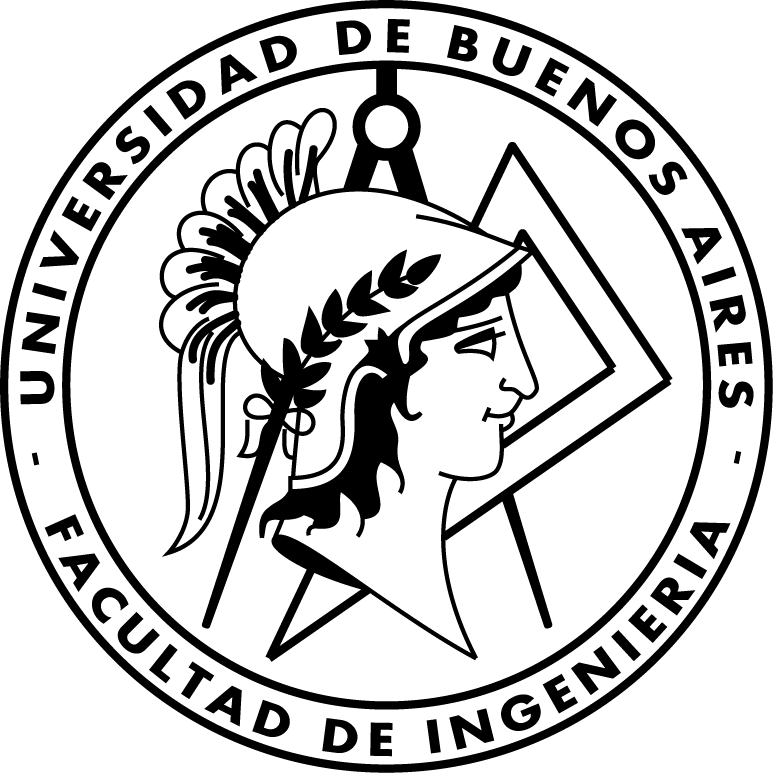
\includegraphics[scale=.4]{./img/Logo-fiuba_big.png}


\medskip
\textbf{\large UNIVERSIDAD DE BUENOS AIRES}

Facultad de Ingenier\'ia

Departamento de Economia, Organizaci\'on y legal


\vspace{3cm}



\textbf{\large 7114 Modelos y Optimizaci\'on 1}

\vspace{2cm}


Este es un modesto aporte para los alumnos de la f\'acultad de ingenier\'ia  de la UBA de las carreras de licenciatura en an\'alsis de sistemas e ingenier\'ia inform\'atica.
De ninguna man\'era pretende ser una gu\'ia de estudio, ni remplaza las clases presenciales, el material oficial de la catedra esta disponible en el web site de la m\'ateria.
\\
wwww.ModelosUno.com.ar

\end {center}


\vspace{2.5cm}

\noindent Autor:	\,Isaac Edgar Camacho Ocampo
 
\noindent Carrera:	\,Licenciatura en An\'alisis de sistemas


\vspace{1cm}

\vspace{1cm}

\noindent Buenos Aires, 2020
\vspace{1cm}
\\
\textit{Si se encuentra alg\'un error u omisi\'on en este res\'umen por favor colaborar en \\
\url{https://github.com/IsaacEdgarCamacho/Apuntes/tree/master/7114 Modelos 1} \quad \\ o escribirme a \\ 
\url{icamacho@fi.uba.ar}
}
\newpage


\tableofcontents
\chapter*{RESUMEN} % si no queremos que añada la palabra "Capitulo"
\addcontentsline{toc}{section}{Resumen} % si queremos que aparezca en el índice
\markboth{RESUMEN}{RESUMEN} % encabezado
El enfoque de la materia se puede dividir en dos partes, y para aprobar, es necesario desarrollar la habilidad de resolver problemas, es por eso que en este apunte, no desarrollaré teoria ni daré definiciones que se pueden hallar en los textos de la materia o en la bibliografía, sino que resolveré la mayor cantidad de ejercicios propuestos en las guías de trabajo, los mismos fuerón resueltos en mi carácter de alumno, de manera que pueden tener errores pero considero que puede ser de utilidad para aquellos estudiantes que cursan por primera vez una materia de programación matemática.
\begin{itemize}
\item Programación lineal continua
	\begin{itemize}
	\item Aprender a modelar problemas complejos
	\item Aprender a resolverlos atravéz del método simplex
	\item Hacer un análisis económico de los resultados obtenidos 
	\end{itemize}
\item Programación lineal Entera
	\begin{itemize}
	\item Aprender a modelar problemas complejos
	\item Problemas combinatorios
	\item Complejidad computacional inherente a esos problemas
	\item Aprender a resolverlos atravéz de métodos como Branch and Bound, Branch and cut y Heuristicas
	\end{itemize}
\end{itemize}

\begin{verse}



La vida nos suele colocar, todo el tiempo, ante la disyuntiva de tener que elegir entre varios caminos. A veces esa libertad de decisión es una experiencia dramática, por las cosas que están en juego.

Es que cada elección trae aparejadas consecuencias, efectos que impactan en uno mismo y en otras personas. En la vida empresarial las decisiones clave descansan en quienes cumplen funciones gerenciales.

La contratación de empleados, la recisión de un contrato con el cliente más importante, la ampliación o remodelación de la línea de producción, la toma de un crédito, por ejemplo, pasa por ellos.

Pero también sobre los gerentes pesan determinaciones dramáticas, como el cierre de la empresa, el llamado a concurso de acreedores, o vender todo y empezar de nuevo.

Y como se sabe, toda decisión entraña un riesgo, porque existe la posibilidad de equivocarse. Es que nadie tiene garantías sobre el futuro, ya que lo que ocurra realmente puede desmentir todos los cálculos.

En este sentido, las decisiones gerenciales pueden llevar al éxito de la organización o a su fracaso. Si son acertadas, garantizan la sustentabilidad y el desarrollo si no, conducen al peor final.

Los expertos definen a la decisión como el resultado de un proceso mental-cognitivo de una persona o de un grupo de individuos. Se conoce como toma de decisiones al proceso que consiste en concretar la elección entre distintas alternativas.

\end{verse}



\chapter{CLASE NRO 1 - INTRODUCCI\'ON.}

\section{Investigación Operativa}
La Investigación Operativa es una disciplina moderna que utiliza modelos matemáticos, estadísticos y algoritmos para modelar y resolver problemas complejos, determinando la solución óptima y mejorando la toma de decisiones. Esta materia también recibe el nombre de Investigación de Operaciones, Investigación Operacional o Ciencias de la Administración.

Actualmente la Investigación Operativa incluye gran cantidad de ramas como la Programación Lineal, Programación No Lineal, Programación Dinámica, Simulación, Teoría de Colas, Teoría de Inventarios, Teoría de Grafos, etc.

\section{Definición aceptada por la SADIO}
La sociedad argentina de Investigación Operativa dice que \'esta es la aplicación de ciencia moderna a problemas complejosque aparecen en la dirección y administración de sistemas constituidos por hombres,
materiales, equipos y dinero en la industria, el comercio, el gobierno y la defensa. Su característica primordial es la elaboración de modelos científicos que mediante la incorporación de factores de riesgo e incertidumbre permitan evaluar decisiones, políticas y alternativas. Su objeto es auxiliar al directivo o al administrativo en la selección científica de susdecisiones.

\section{Mod\'elos}
\subsection{¿Que es modelizar?} Es hacer una simplificacion de la realidad y nosotros trabajamos con esa simplificacion ya que la realidad es muy compleja.
\subsection{¿Para que hacer un modelo?}
\begin{itemize}
\item \textbf{Economia de recursos:} Al igual que en la ingenieria civil cuando se hacen planos para representar una obra (ya que no seria l\'ogico hacer el edificio y ante un error rehacerlo), cuando modelamos un problema usando programacion lineal y dada la escazes de recursos, es mas eficiente trabajar sobre modelos.
\item \textbf{Eficiencia}: de nuevo so no tengo recursos limitantes entonces trabajo sobre la realidad y no modelo nada.
\item \textbf{simplicidad}: puedo mediante abstracci\'on lograr un modelo mas sencillo y eliminar la complejidad inherente del problema.
\item \textbf{En resumen es mejor que hacer multiples ensayos.}
\end{itemize}
Los mod\'elos se aplican a problemas de desici\'on y este existe cuando existen formas alternativas de actuar, con distintos resultados y diferentes eficiencias para lograr el objetivo es decir existen dudas respecto del curso alternativo a utilizar.


\section{Elementos de un modelo}
\subsection{Hipótesis y supuestos:} Para simplificar el modelo se delimita el sistema en estudio a través de las hipótesis y
supuestos simplificativos. Así se comienza a transformar el sistema físico en un modelo simbólico.
Las hipótesis deben ser probadas científicamente. Los supuestos son hipótesis que no pueden probarse.

\textbf{Ejemplos:}
Si estamos modelando una panaderia, y el recurso agua no es limitante y por otro no se dice nada de 				la venta de lo producido podemos agregar las hipotesis
\begin{enumerate}
	\item 	
	\textit{Hay agua suficiente para todos los procesos}
	\item
	\textit{Se vende todo lo que se produce}
\end{enumerate}
\subsection{Objetivo: }Mide la eficiencia de nuestro sistema y lo que buscamos es hallar la merjo solucion. El objetivo surge como respuesta a tres preguntas:
\\¿Qué hacer? es decir que es lo que queremos determinar.
\\¿Cuándo? (período de tiempo) puede ser un mes o año o un periodo t si no se especifica.
\\¿Para qué? para maximizar ganancias, o minimizar costos, nunca ambos a la vez.
\subsection{Actividad}
Proceso unitario que se realiza en el sistema físico caracterizado por consumir recursos
y/o generar un resultado económico y/o indicar un estado, por ejemplo producir un bien o indicar si se finaliz\'o un proceso.
\subsection{Variables}
Son las que miden o indican el estado de una actividad.
Las que miden pueden ser continuas o enteras.
Las que indican son, generalmente, variables (0,1) o bivalentes

\section{Programación lineal}La programación lineal es el campo de la programación matemática dedicado a maximizar o minimizar una función lineal, denominada función objetivo, de tal forma que las variables de dicha función estén sujetas a una serie de restricciones expresadas mediante un sistema de ecuaciones o inecuaciones también lineales.
\subsection{Programación Lineal Continua}
\subsection{Programación Lineal Entera}Es una tecnica que permite modelar y resolver problemas cuya caracterıstica principal
es que el conjunto de soluciones factibles es discreto.
\\
\\

\begin{itemize}
\item \textbf{OR l\'ogico}
\[ Y_{or} \quad \leq \quad \sum_{i=1}^{n}Y_{i} \quad \leq \quad n Y_{or}\]
\item \textbf{AND l\'ogico}
\[ n Y_{and} \quad \leq \quad \sum_{i=1}^{n}Y_{i} \quad \leq \quad (n-1) + Y_{and} \]
\end{itemize}


\subsection{Supuestos básicos de la Programación Lineal Continua}
\subsubsection{Proporcionalidad}
Tanto el beneficio como el uso de recursos son directamente proporcionales al nivel de
actividad
\subsubsection{Aditividad}No existen interacciones entre las actividades que cambien la medida total de la
efectividad o el uso total de algún recurso
\subsubsection{Divisibilidad}Las unidades de actividad pueden dividirse en niveles fraccionarios cualesquiera, de
modo que pueden permitirse valores no enteros para las variables
\subsubsection{Certeza}Todos los parámetros del modelo son constantes conocidas

\section{Centros de producción}
\subsection{Armado vs Mezcla}

\section{Conceptos previos}
\begin{enumerate}
	\item \textbf{Eficiencia:} Producir mas con menos recursos o productividad.
	\item \textbf{Eficacia:} Lograr el resultado aunque se consuman muchos recursos.
	\item \textbf{Costo de oportunidad:} Es el costo de producir una unidad de un bien.
	\item \textbf{Contribucion marginal:} Ganancia neta.
\end{enumerate}

\section{Primer caso de estudio}

La panadería la Higiénica elabora en forma absolutamente artesanal y con elementos orgánicos, baguettes y pan de campo.\\
Los ingredientes principales son harina, agua,sal y levadura. Para hacer una baguette hacen falta 100 gr de harina, 60 cc de agua, 10 gr de levadura y para hacer un pan de campo hacen falta 250 gr de harina, 200 cc de agua, 12 gr de levadura. \\
Usa harina integral y cuenta con 100 kg, el agua la traen desde Mendoza y tiene 80 litros, de levadura hay 8 kg. La sal es marina y tiene una bolsa de 50 kg. \\
Las baguettes se entregan en bolsitas de papel de las que tiene 450 unidades.
Las ganancias unitarias son de \$0.30  y de \$0.80  para las baguettes y los panes respectivamente.
Se quiere programar el trabajo del día de mañana.





\chapter{Práctica 1 - Conjuntos, Relaciones y Funciones}
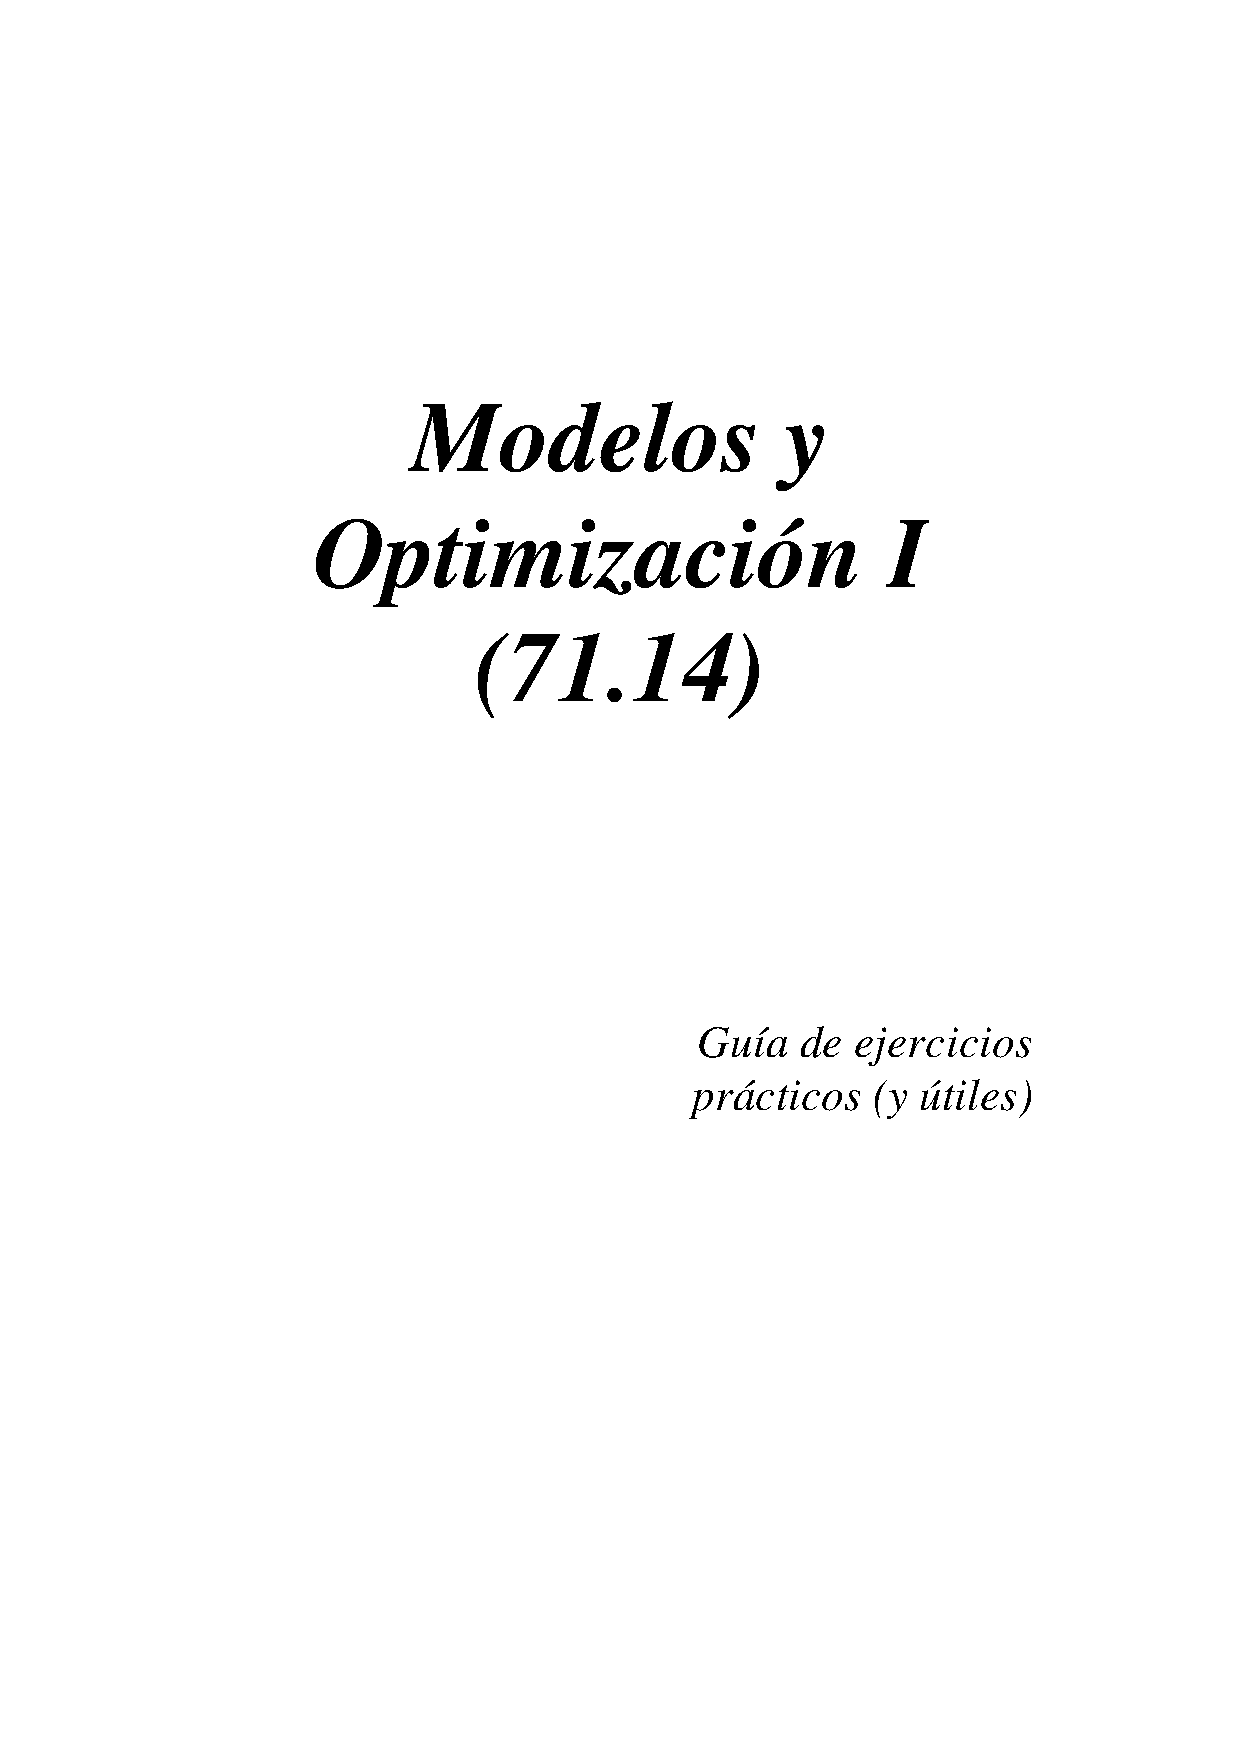
\includepdf[pages=-]{./pdfs/GuiaTP_Cap1.pdf}

\section{Resoluci\'on Guia 1}
Toda la guía 1 se trata de resolver problemas de programación lineal continua, son problemas sencillos de planificación de producción con restricciones de demanda mínima o recursos limitados, resolver los ejercicios significa plantear el modelo matemático con todos sus elementos, no hay que hallar la solucion exacta, eso lo haremos con el algoritmo simplex más adelante.

\subsection{Ejercicio 1.1}
\textbf{Objetivo: }determinar la cantidad de productos A y B a fabricar en un mas para maximizar las ganancias.
\\
\textbf{Hip\'otesis: }
\begin{enumerate}
\item no existen m\'ermas en el proceso de producci\'on.
\item todo lo que se produce se vende, es decir que la demanda no es limitante.
\item no existe acumulaci\'on de stock.
\end{enumerate}

\textbf{Variables :}
\begin{itemize}
\item $P_a [\frac{unidades}{mes}]$: cantidad fabricada de producto tipo A
\item $P_b [\frac{unidades}{mes}]$: cantidad fabricada de producto tipo B 
\end{itemize}
\textbf{Inecuaciones: }
\begin{itemize}
\item $3 [\frac{m^3}{unidad}]  P_a[\frac{unidades}{mes}] + 2/3 [\frac{m^3}{unidad}]  P_b [\frac{unidades}{mes}] \geq 40 [\frac{m^3}{mes}]  $ \, \textit{(Consumo de alcohol)}

\item $1 [\frac{ton}{unidad}]  P_a[\frac{unidades}{mes}] + 2 [\frac{ton}{unidad}]  P_b [\frac{unidades}{mes}] \leq 20 [\frac{ton}{mes}]  $ \, \textit{ (Consumo de ciclohexano)}
\end{itemize}
\pagebreak
\textbf{Funcional: }El funcional hace que las variables $P_a$ y $P_b$ tomen valores lo m\'as grandes posibles teniendo en cuenta que el ciclohexano tiene un l\'imite en su disponibilidad y por otro lado el alcohol tiene un consumo m\'inino.
\begin{itemize}
\item $Z_{max} \Rightarrow 1200 [\frac{\$}{unidad}]  P_a[\frac{unidades}{mes}] + 400 [\frac{\$}{unidad}]  P_b [\frac{unidades}{mes}] $
\end{itemize}

\begin{center}
\textbf{Resoluci\'on gr\'afica}
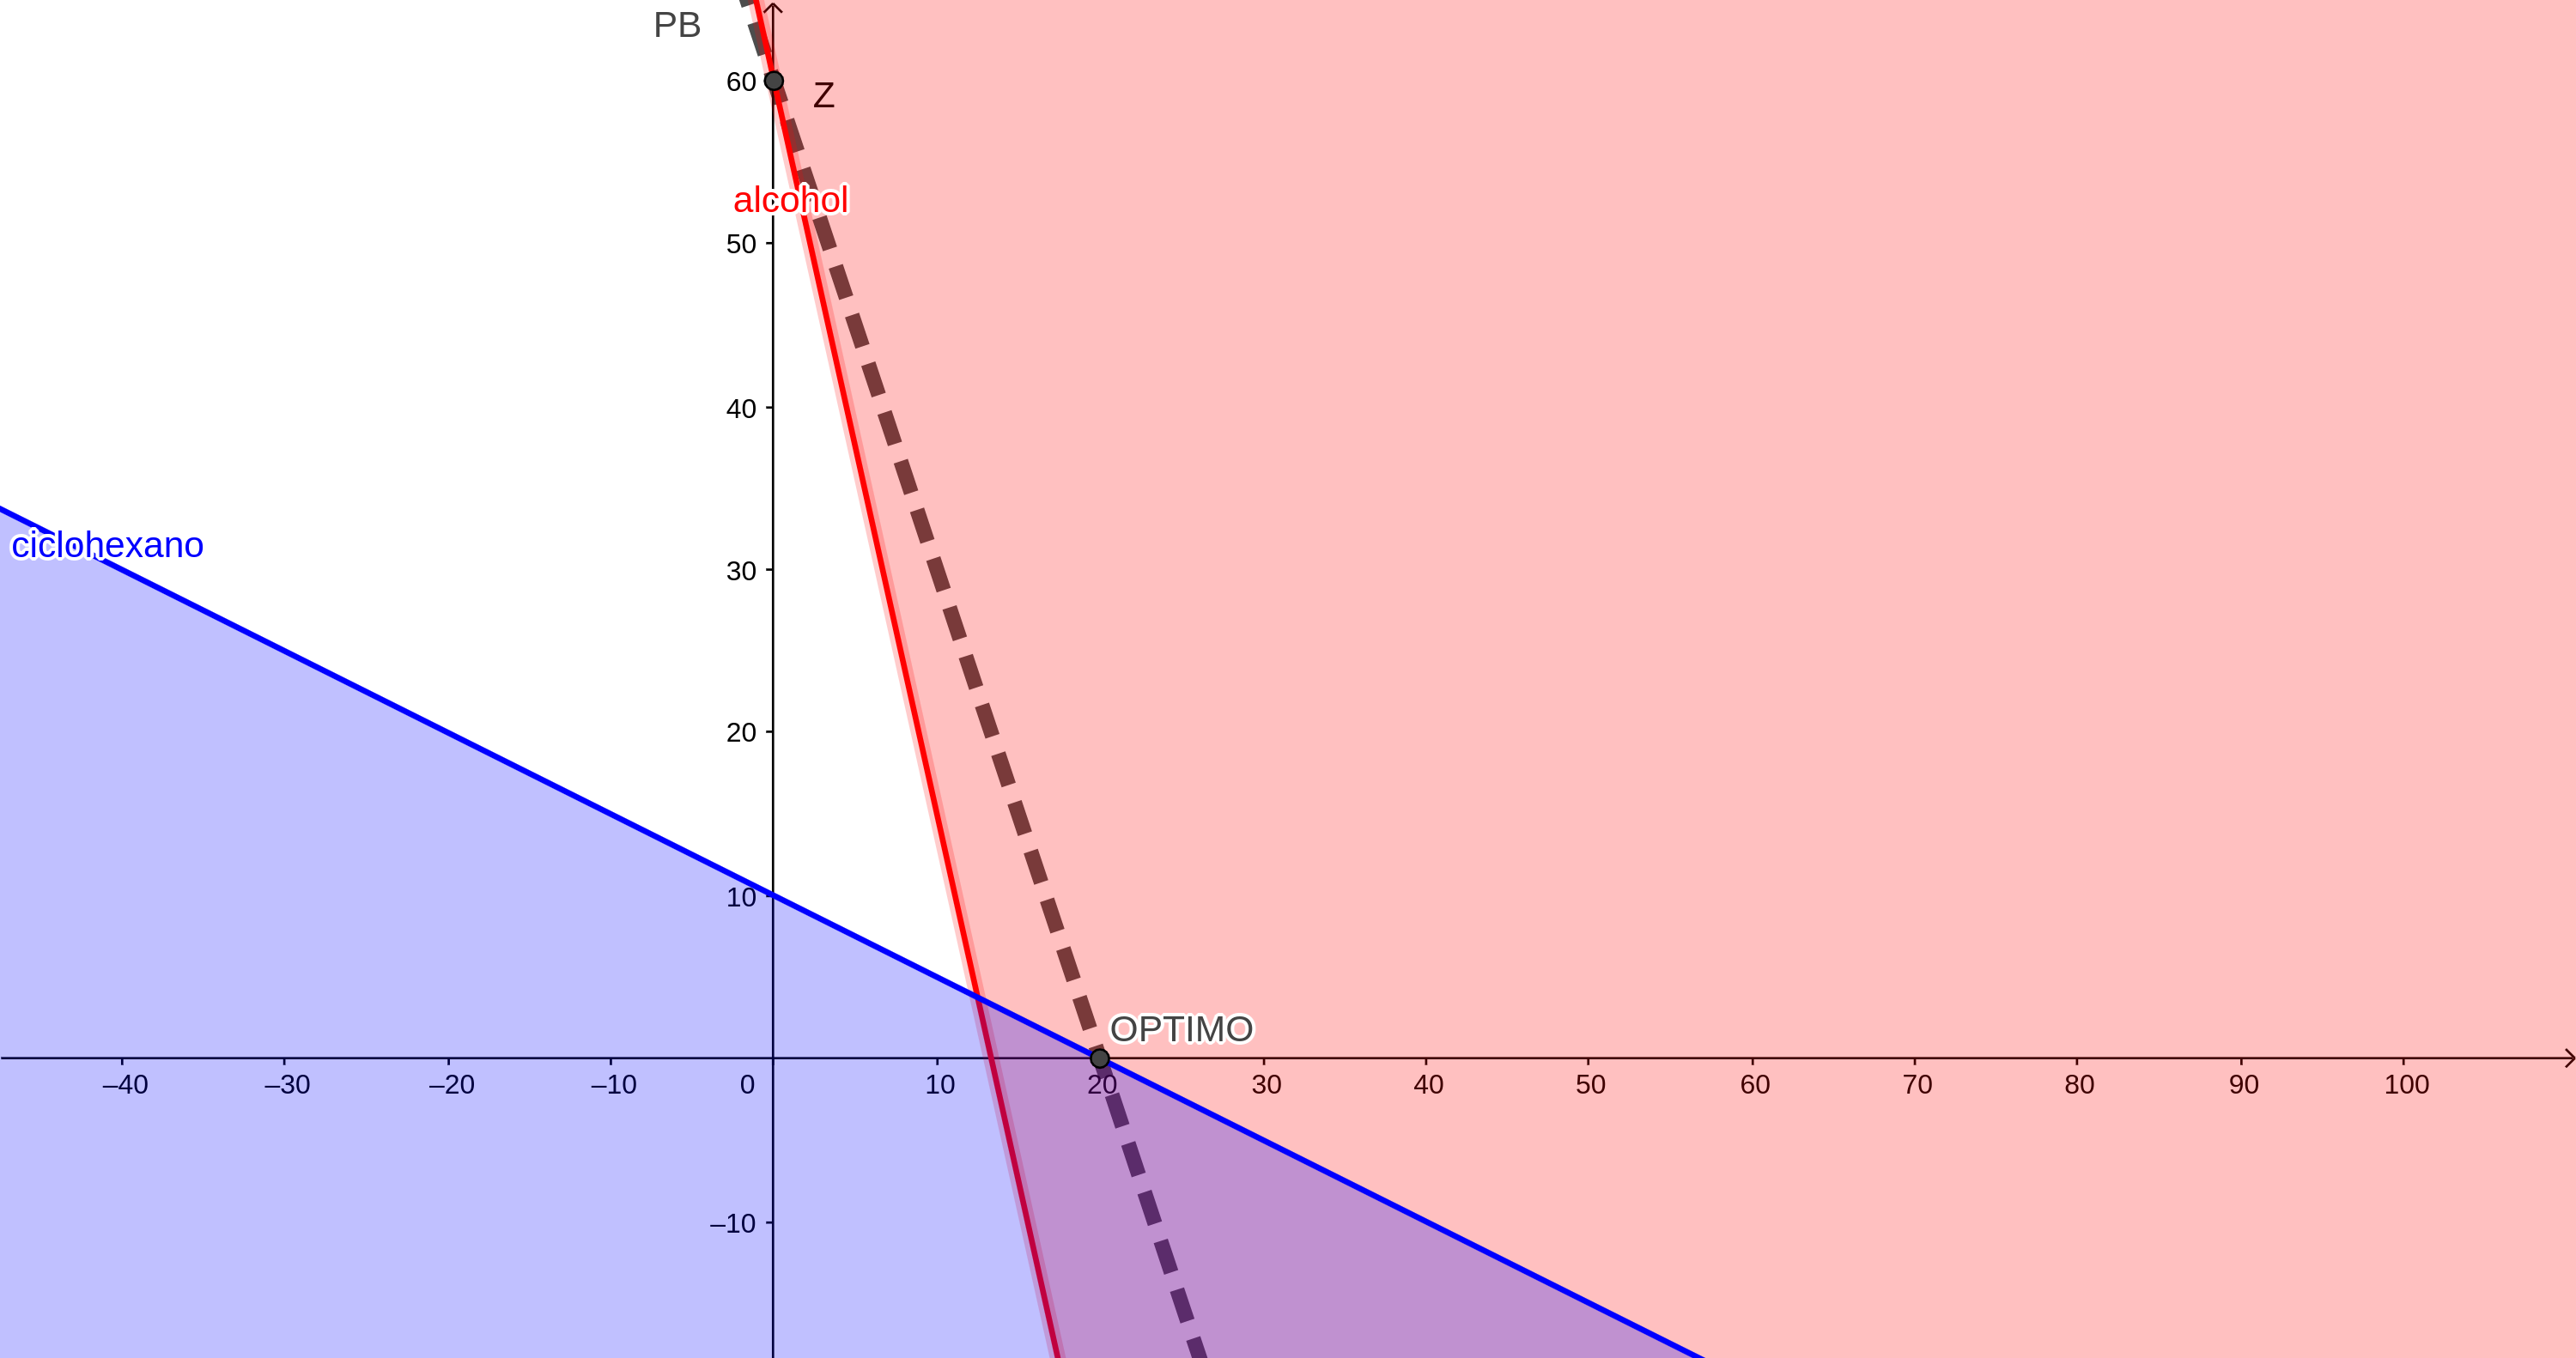
\includegraphics[scale=.1]{./img/1-1.png}
\end{center}


\subsection{Ejercicio 1.2}
\textbf{Hipótesis}
\begin{enumerate} 
\item No existen mermas de producción.
\item No existen stocks.
\item Se vende todo lo producido.
\end{enumerate}

\textbf{Variables}
\begin{itemize}
\item P1 $[un/mes]$ (unidades de producto 1 producidos en un mes)
\item P2 $[un/mes]$ (unidades de producto 2 producidos en un mes)
\end{itemize}

\textbf{Objetivo}
Determinar la producción de P1 y P2 en un mes de trabajo para maximizar las ganancias.
\\ \\ \\
\textbf{Modélo}
\begin{align*}
2 P1 + 4 P2 &\leq 80 [hs/mes] \\
3 P1 + 2 P2 &\leq 60 [hs/mes] \\
4 P1 + 2 P2 &\leq 100 [hs/mes] \\
Funcional \quad Z_{max} \Rightarrow  60 P1 &+ 50 P2 
\end{align*}

\begin{center}
\textbf{Resoluci\'on gr\'afica}
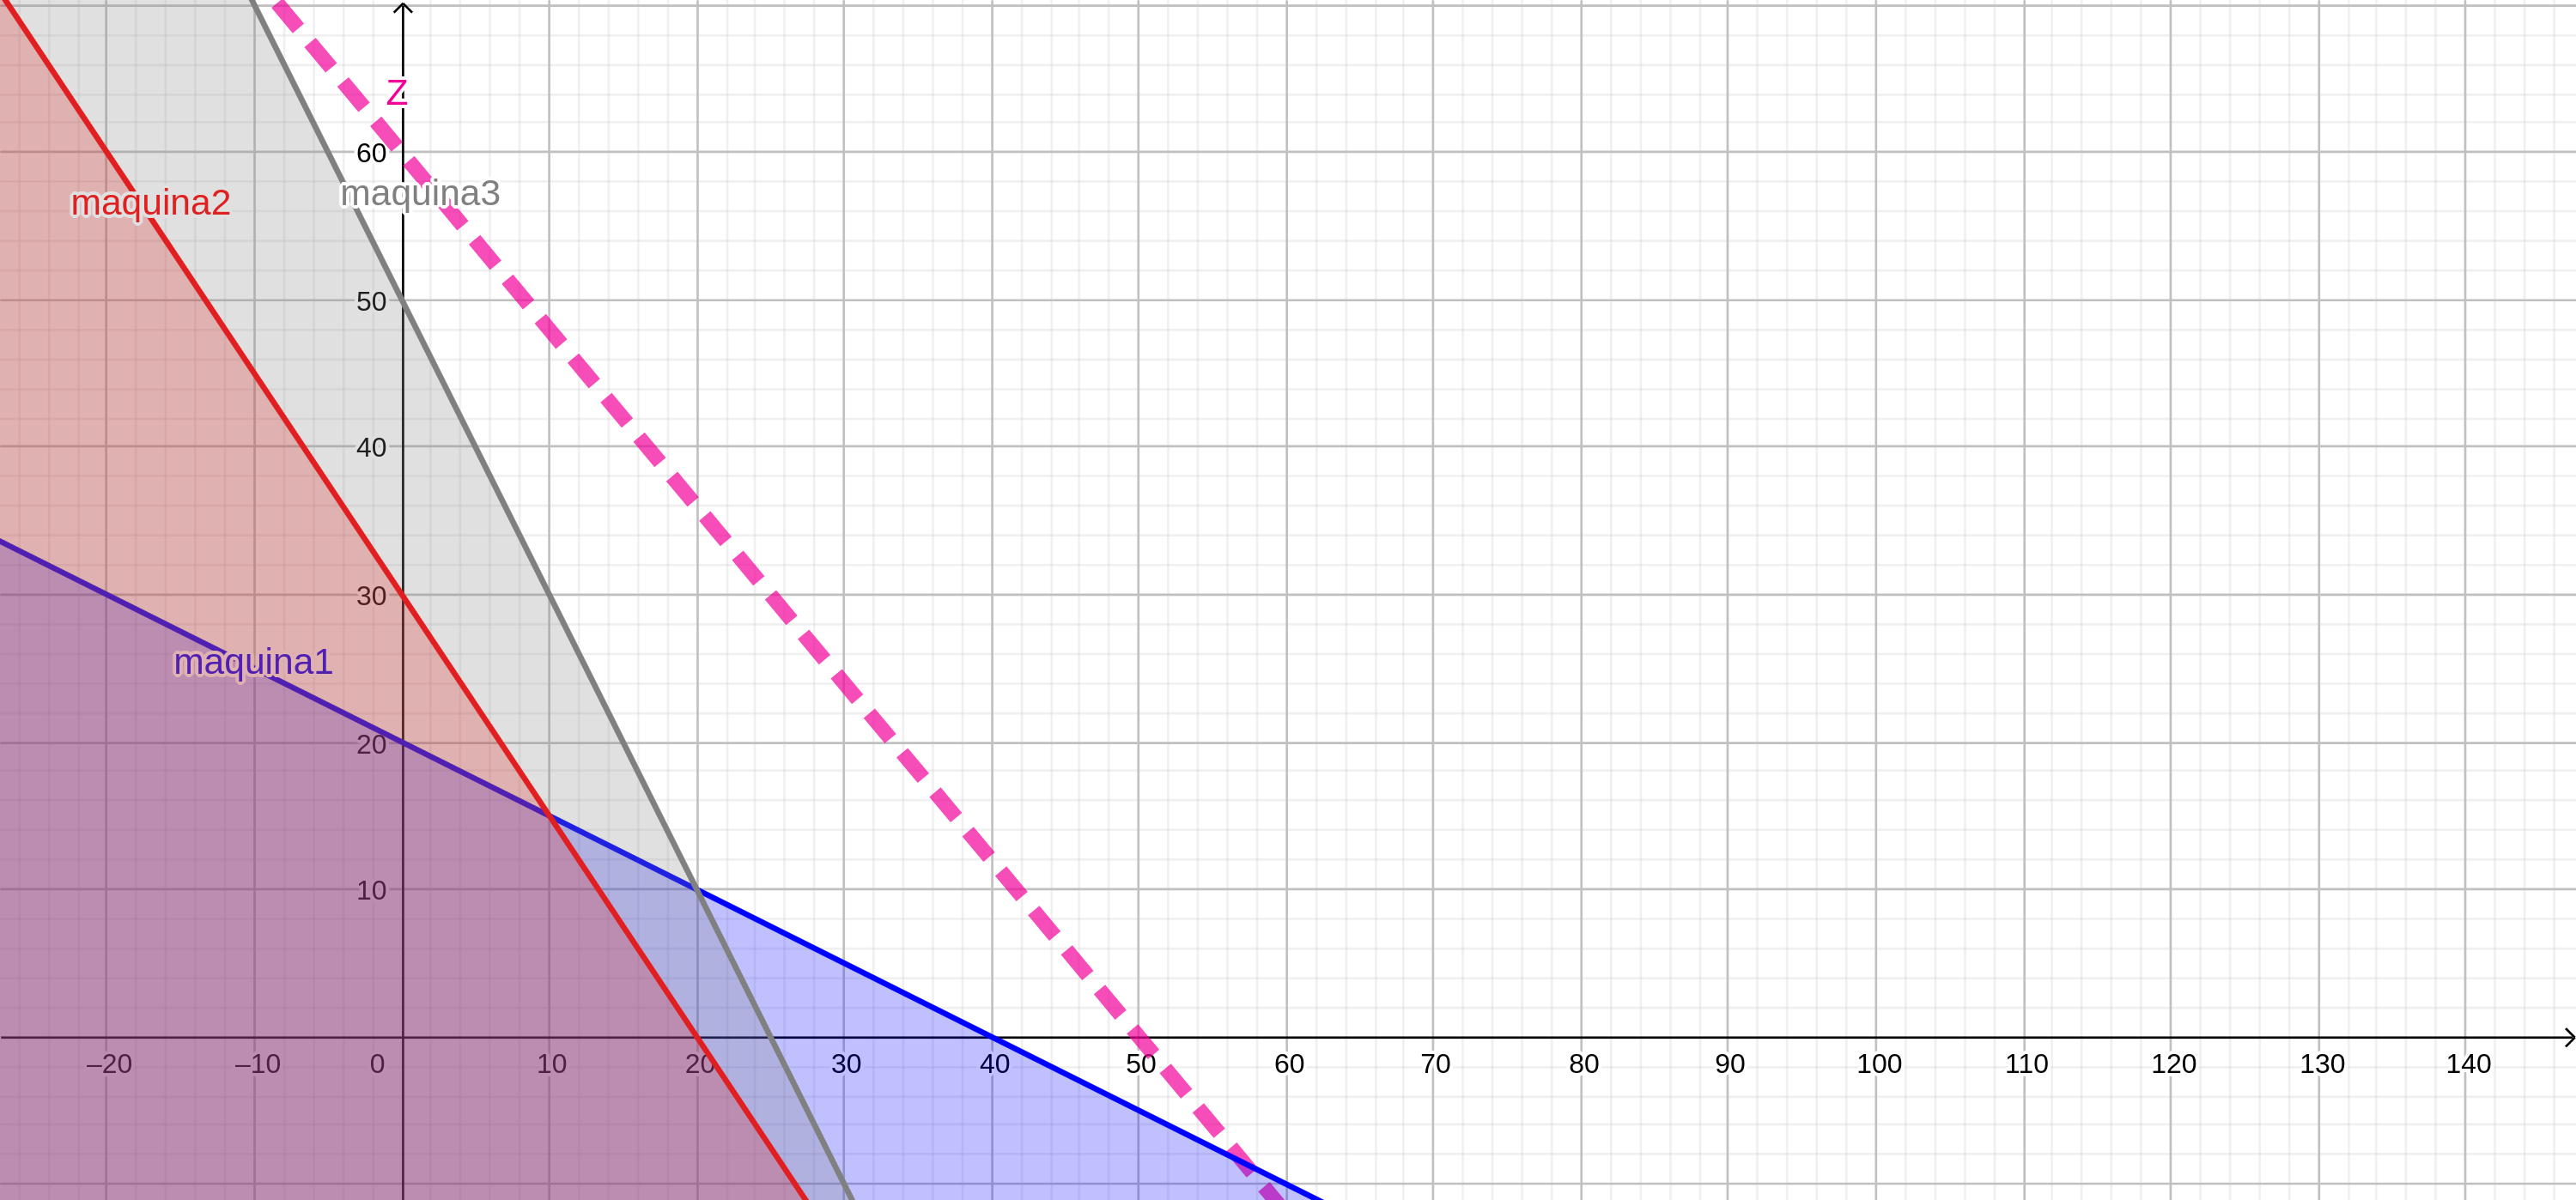
\includegraphics[scale=.1]{./img/geogebra-export.png}
\end{center}
Respecto de la pregunta final, si, es conveniente conseguir mas recurso porque si nos fijamos en el gráfico el equipo 2 es limitante ya que el óptimo esta sobre su recta, conseguir mas recurso implica que dicha récta se va a relajar es decir, se va a alejar del origen lo que significa que el funcional sera mayor.





\subsection{Ejercicio 1.3}
\textbf{Hipótesis}
\begin{enumerate} 
\item No existen mermas de producción.
\item No existen stocks.
\item Se vende todo lo producido.
\end{enumerate}

\textbf{Variables}
\begin{itemize}
\item PA $[un/T]$ (unidades de producto 1 producidos en un período indeterminado T)
\item PB $[un/T]$ (unidades de producto 2 producidos en un período indeterminado T)
\end{itemize}

\textbf{Objetivo}
Determinar la producción de PA y PB en un tiempo de trabajo T para maximizar las beneficios.

\textbf{Modélo}
\begin{itemize}
\item $1 PA + 0,4 PB \leq 200 $ (disponibilidad de maquina A)
\item $0,5 PA + 1 PB \leq 200 $ (idem maquina B)
\item $ PA \geq 50 $ (Pedido mínimo de producto A)
\item $ PB \geq 4 PA $ (La produccion de B es 4 veces la de A)
\item Funcional $ Z_{max} 12 PA + 8 PB $ 
\end{itemize}

\begin{center}
\textbf{Resoluci\'on gr\'afica}
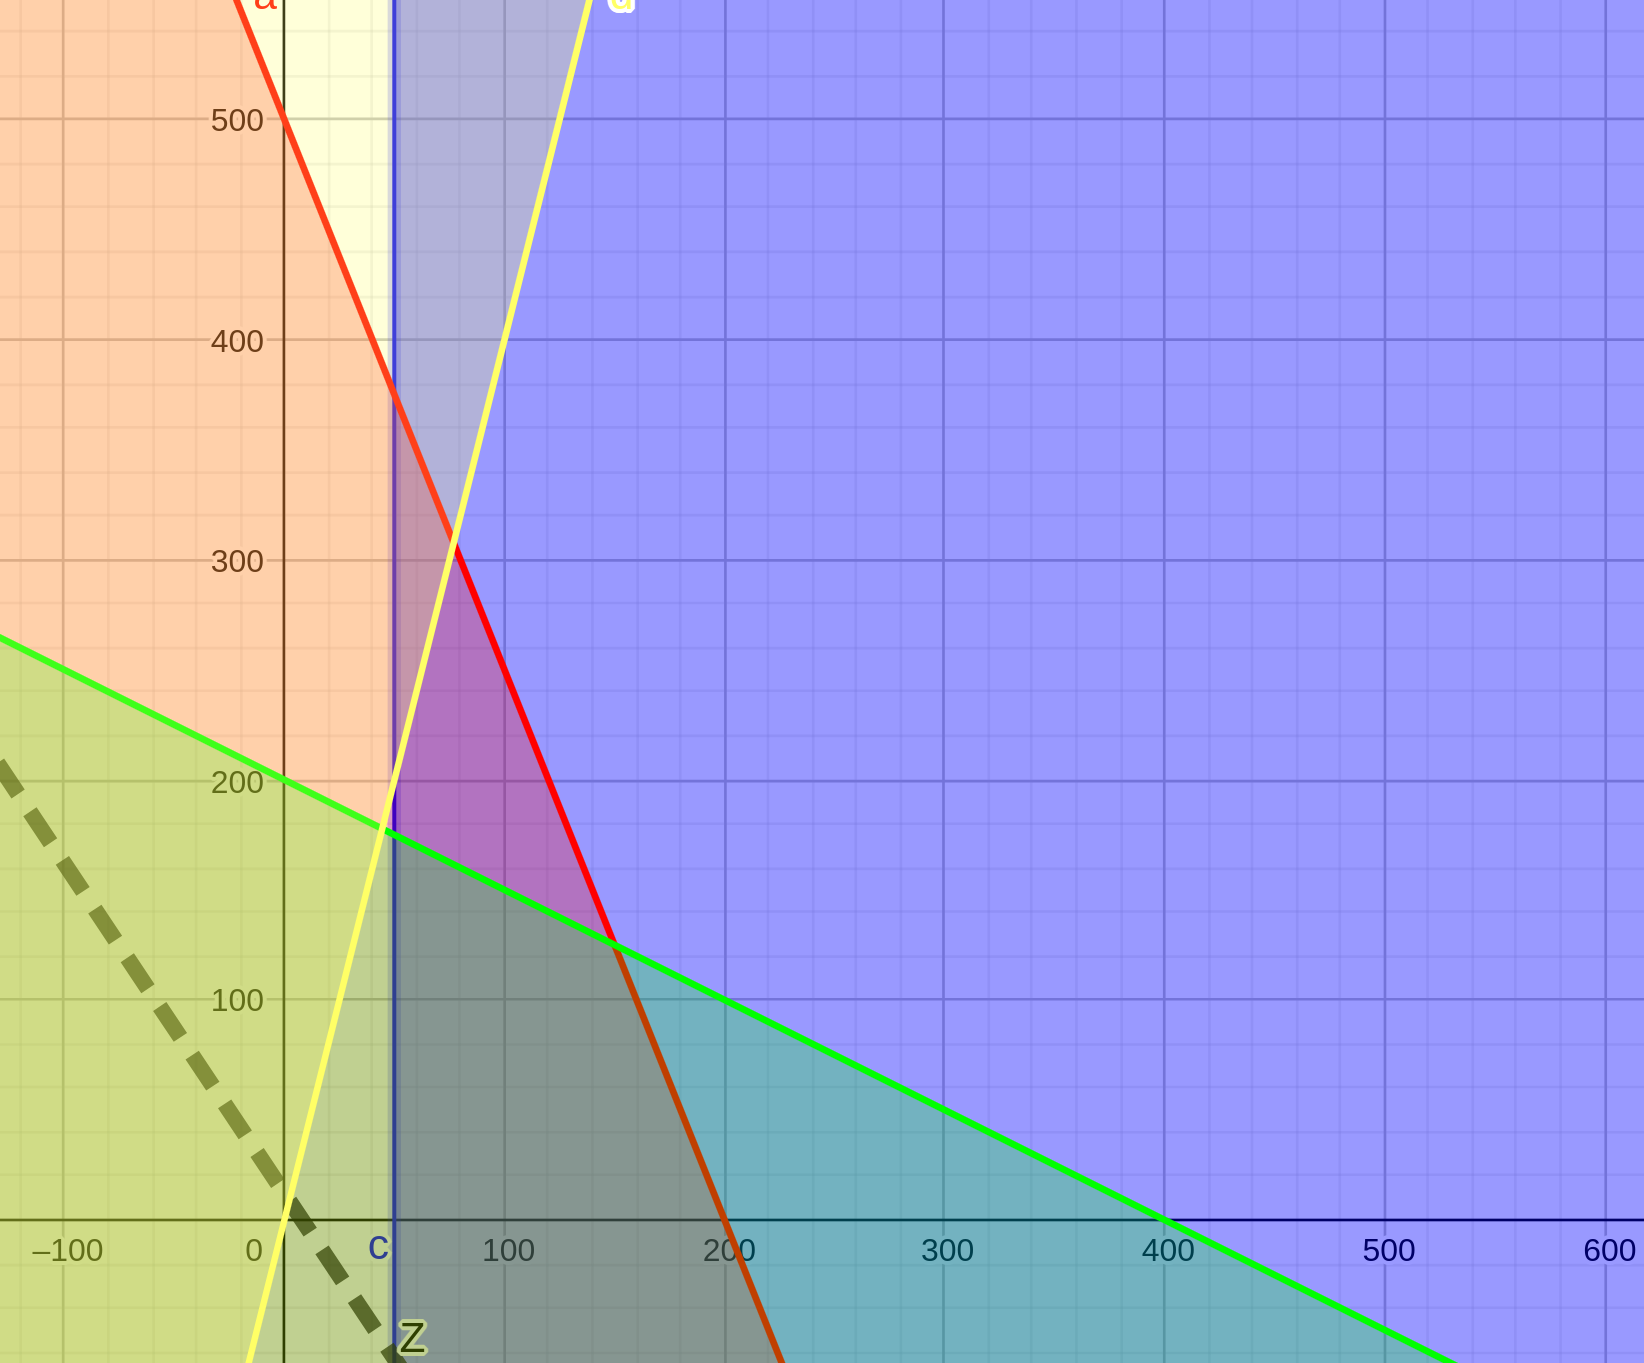
\includegraphics[scale=.3]{./img/13.png}
\end{center}




\subsection{Ejercicio 1.4}
Este ejercicios nuevamente se trata de planificación de la producción el tiempo es de una semana de trabajo y hay recursos limitantes.
\\
\textbf{Hipótesis}
\begin{enumerate} 
\item El dato de 90\% no inside en el modelo
\item No existen stocks.
\item Se vende todo lo producido.
\item Como nada se dice de los costos, suponemos que estan incluidos en el precio de venta.
\end{enumerate}

\textbf{Variables}
\begin{itemize}
\item Mred $[un/sem]$ (manteles redondos)
\item Mrec $[un/mes]$ (manteles rectangulares producidos en una semana)
\end{itemize}

\textbf{Objetivo}
Determinar la producción de los dos tipos de manteles en un una semana de trabajo para maximizar las ganancias.
\\ \\ \\
\textbf{Modélo}
\begin{align*}
2 Mred + 3 Mrec &\leq 600 [m^2/sem] \\
3 Mred + 1 Mrec &\leq 500 [hs/sem] \\
4 Mrec &\leq 600[esq/sem] \\
Funcional \quad Z_{max} \Rightarrow  8 Mred &+ 10 Mrec
\end{align*}

\begin{center}
\textbf{Resoluci\'on gr\'afica}
%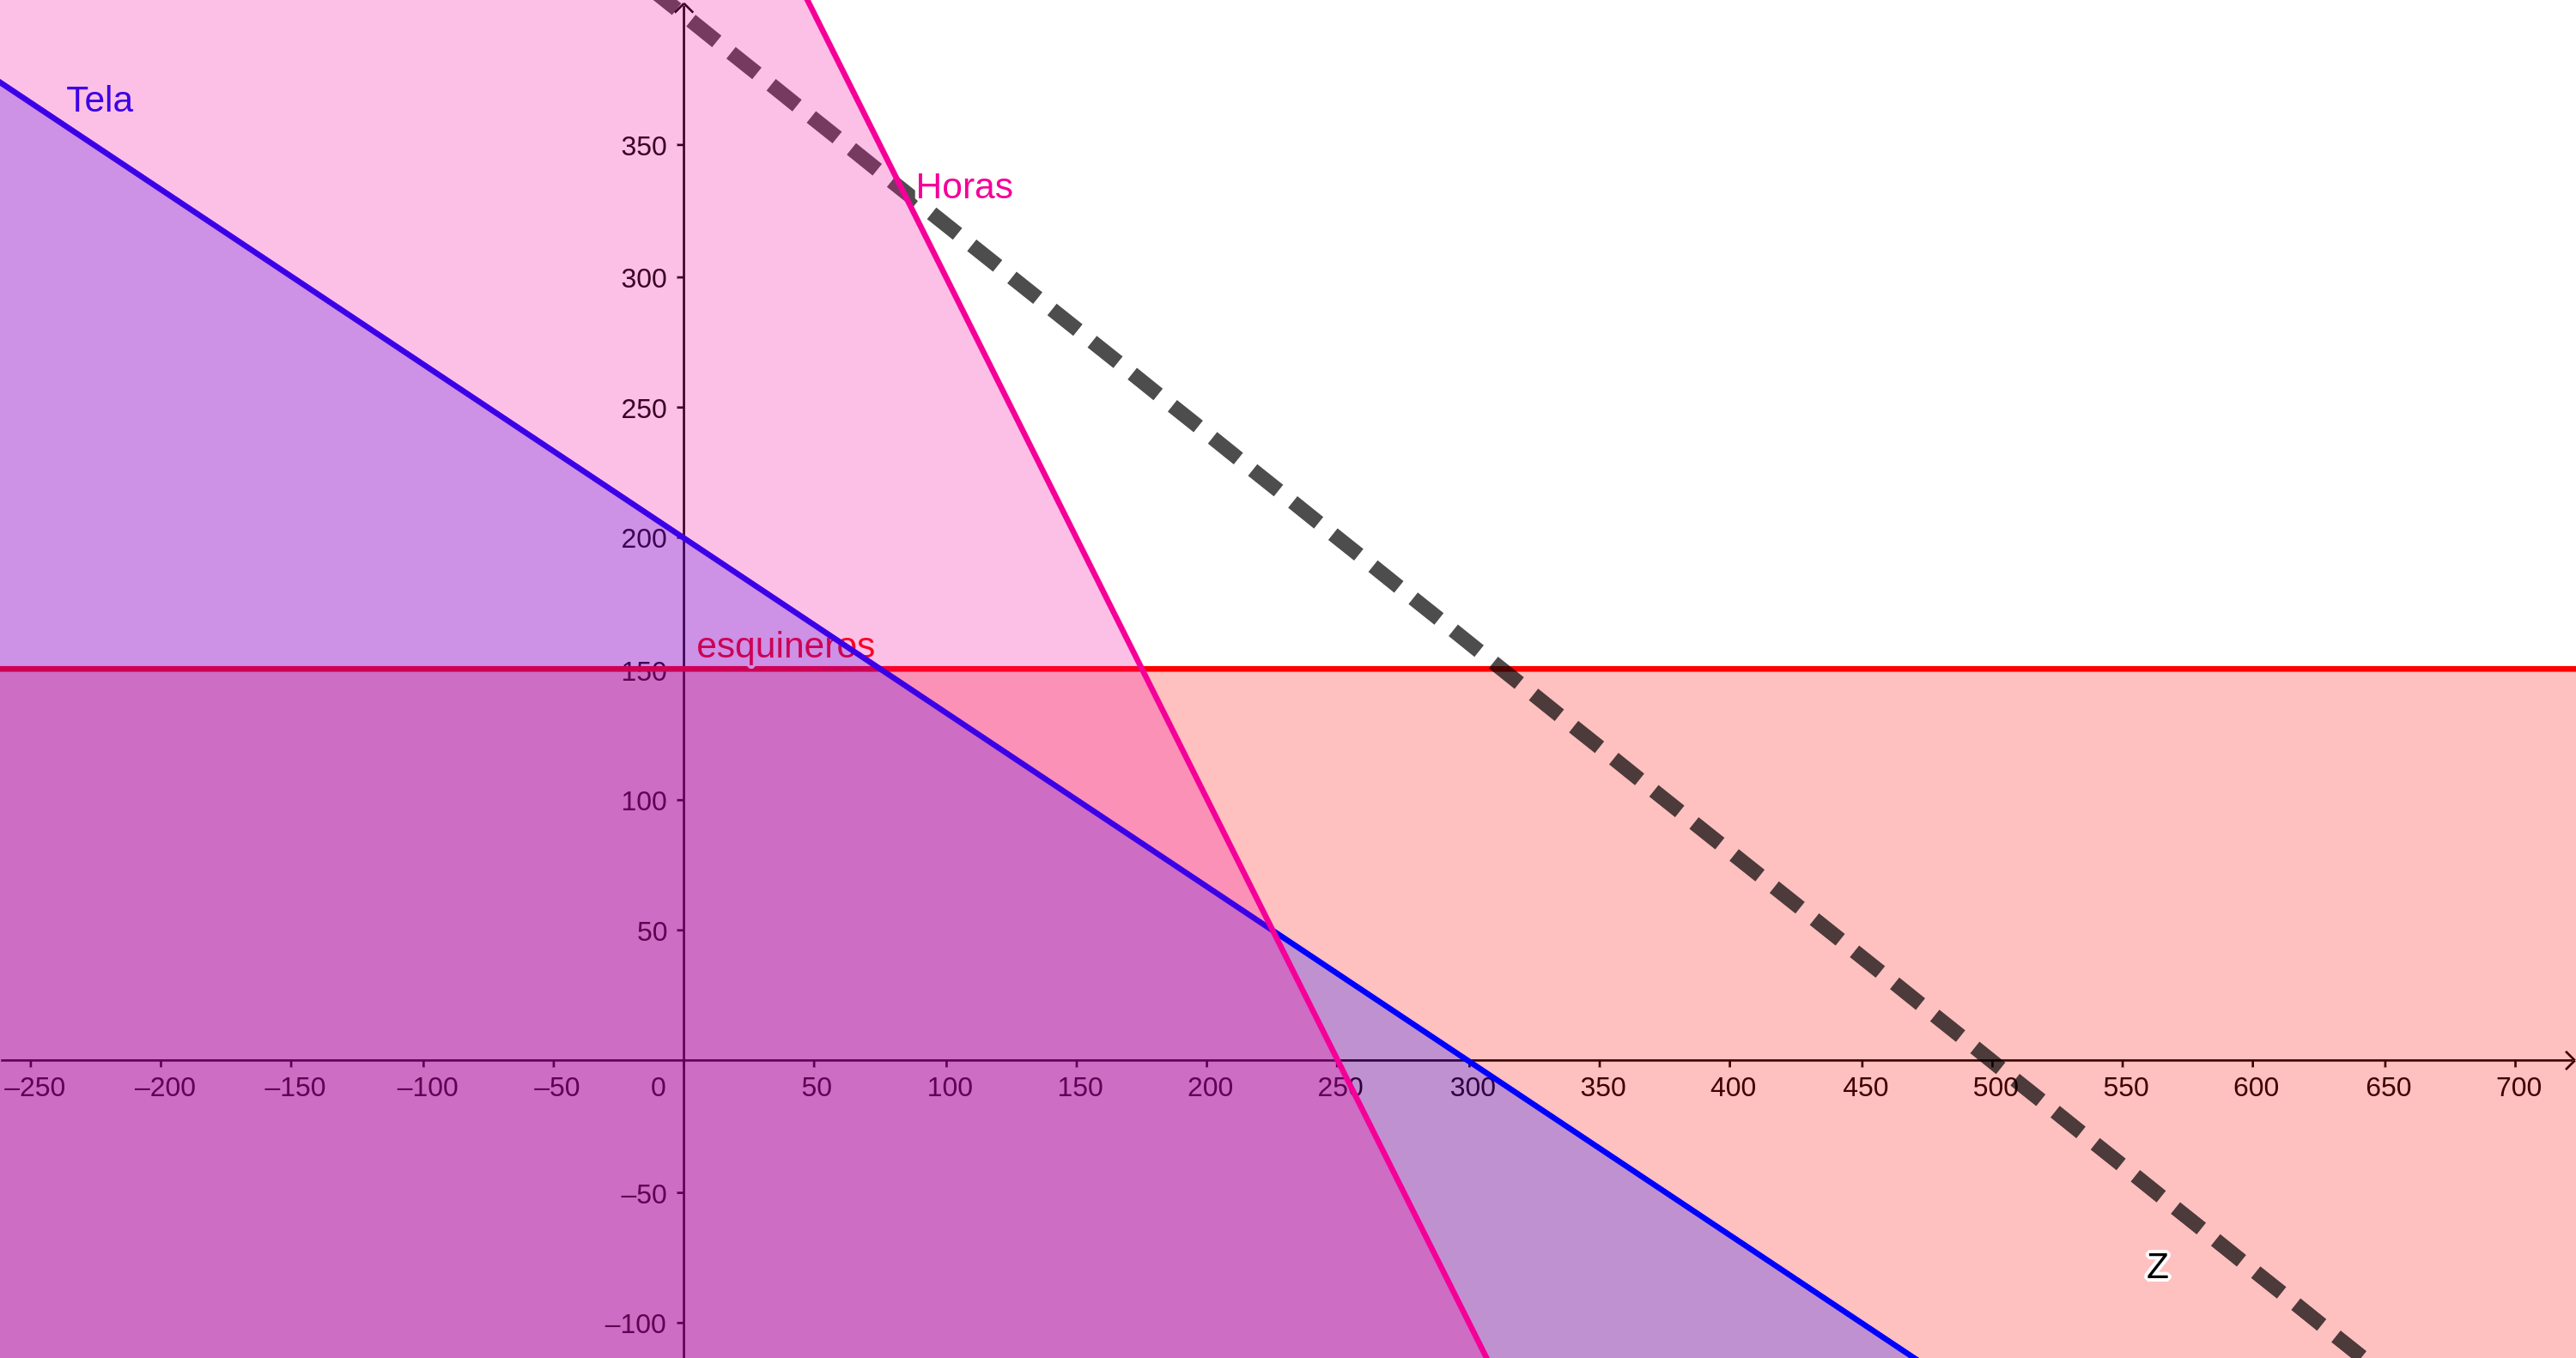
\includegraphics[scale=.1]{./img/14.png}
\end{center}



\chapter{Práctica 2 - Conjuntos, Relaciones y Funciones}

\includepdf[pages=-]{./pdfs/GuiaTP_Cap2.pdf}

\section{Resoluci\'on Guia 2}
En esta guía las variables que manejamos ya no son dos y la principal consecuencia es que ya no podremos representar gráficamente nuestro modelo,  De manera que no podemos calcular gráficamente el punto óptimo, Nuestro trabajo será simplemente modelar el problema sin resolverlo por ahora 

\subsection{Ejercicio 2.1}
Podemos observar el incremento en la complejidad del problema a modelar, aquí ya no son dos productos sino tres y además se incorporan otros factores como la producción del pullover tipo b que se puede hacer en dos máquinas, también tenemos demanda mínima del pullover tipo B.

Aquí tenemos un primer esbozo de productos enteros es decir los pulóveres no se venden en partes, es una unidad, es importante la hipótesis que nos dice que los pulóveres pueden quedar a medio terminar de lo contrario tendríamos que modelar utilizando programación entera.
\\ \\
\textbf{Objetivo: }determinar la cantidad de pulloveres de tipo A, B y C a fabricar en una semana para maximizar las ganancias.
\\
\textbf{Hip\'otesis: }
\begin{enumerate}
\item no existen m\'ermas en el proceso de producci\'on.
\item todo lo que se produce se vende, es decir que la demanda no es limitante.
\item no existe acumulaci\'on de stock inicial.
\item todas las materias primas son de 1º calidad.
\item los costos estan contemplados.
\end{enumerate}

\textbf{Variables :}
\begin{itemize}
\item $P_i [\frac{unidades}{sem}] \quad i \epsilon [A,B,C]$: cantidad fabricada de pullover tipo i
\end{itemize}

\textbf{Inecuaciones: }
Las dos máquinas trabajan dos turnos por día, 8 horas en cada turno, de lunes a viernes, traducido a horas son 80 horas por semana.
\begin{itemize}
\item $P_B = P_{B1} + P_{B2} $ debemos saber cuantos pullovers tipo B se hace con cada maquina.
\item $5 [\frac{hs}{un}]  P_A [\frac{unidades}{sem}] + 6 [\frac{hs}{unidad}]  P_{B1} [\frac{unidades}{sem}] \leq 80 [\frac{hs}{sem}]  $ \, \textit{(Consumo máquina 1)}

\item $4 [\frac{hs}{unidad}]  P_{B2}[\frac{unidades}{sem}] + 4 [\frac{hs}{unidad}]  P_C[\frac{unidades}{mes}] \leq 80 [\frac{hs}{sem}]  $ \, \textit{ (Consumo máquina 2)}
\item $1,6 P_A +1,2 P_C \leq 20 [kg /sem]$ (Disponibilidad de lana mejorada)
\item $1.8 PB \leq 36 [kg /sem] $ (lana normal)
\item $ P_B \geq 10 [un/sem]$ (demanda mínima de pullovers B)
\end{itemize}
\pagebreak
\textbf{Funcional:} 
\begin{itemize}
\item \[ Z_{max} \Rightarrow 10[\frac{\$}{unidad}]  P_A[\frac{unidades}{sem}] + 15 [\frac{\$}{unidad}]  P_B [\frac{unidades}{sem}] + 18 [\frac{\$}{unidad}]  P_C [\frac{unidades}{sem}] \]
\end{itemize}



\subsection{Ejercicio 2.2}
Aquí podemos ver un problema tipo parcial, es un proceso productivo que consiste en la extracción de un mineral que contiene 4 metales y luego producir dos aleaciones, la extracción está disponible en 3 yacimientos, y tienen un costo asociado y una composición diferente en lo respectivo a los metales que contiene, es conveniente hacer un esquema para resumir la información disponible.
\\
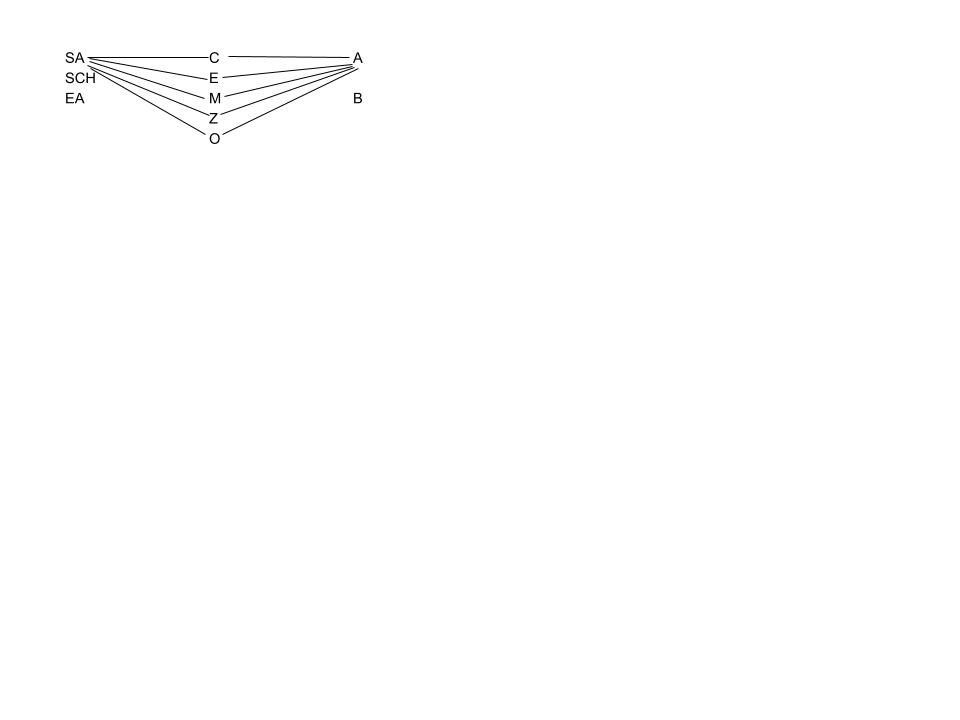
\includegraphics[scale=.9]{./img/IMG2-2.png}



\textbf{Objetivo: }Determinar el plan de producción de aleaciones tipo A y B en un tiempo indeterminado T, teniendo en cuenta las disponibilidades de materia prima en cada yacimiento asi como el costo de extracción, con el objetivo de maximizar los beneficios.
\\
\textbf{Hip\'otesis: }
\begin{enumerate}
\item no existen m\'ermas en el proceso de producci\'on.
\item todo lo que se produce se vende, es decir que la demanda no es limitante.
\item todas las materias primas son de 1º calidad.
\end{enumerate}

\textbf{Variables :}
Vamos a tener que abrir las variables, debido a que tenemos que determinar cuantos metales se extraen de cada yacimiento, tambien debemos abrir las variables para saber cuanto usamos en cada aleacion.
\begin{itemize}
\item $ A , B [\$/ton] $ (aleación de tipo A y B)
\item $ C_{sa}, E_{sa}, M_{sa}, Z_{sa}, O_{sa} $ (cobre que proviene del yacimiento sierra alta, idem los demas)
\item $ C_A, E_A, M_A, Z_A,O_A $ (Cobre que va a la aleación A, idem para los demas.)
\item $ MSA [ton /T] $ (toneladas de mineral extraidos de sierra alta, idem para los demás)
\end{itemize}

\textbf{Inecuaciones: }

\begin{itemize}
\item $ MSA = C_{sa} + E_{sa} + M_{sa} + Z_{sa} + O_{sa} \leq 1000 [ton/T]$ (disponibilidad en sierra alta)
\item $ MSCH = C_{sch} + E_{sch} + M_{sch} + Z_{sch} + O_{sch} \leq 2000 [ton/T]$
\item $ MEA = C_{ea} + E_{ea} + M_{ea} + Z_{ea} + O_{ea} \leq 3000 [ton/T]$
\item Extracción en sierra alta
	\begin{itemize}
	\item $ 0,2 MSA = C_{sa}$ (el 20\% del mineral extraido de SA es cobre)
	\item $ 0,1 MSA = E_{sa}$
	\item $ 0,3 MSA = M_{sa}$	
	\item $ 0,3 MSA = Z_{sa}$	
	\item $ 0,1 MSA = O_{sa}$ (el 10\% es de otros metales)	
	\end{itemize}
	se plantean identicas ecuaciones para cada yacimiento con sus respectivos porcentajes.
\item Proceso de Aleación, este es un proceso de mezcla ya que no podemos distinguirlo en el producto final.
	\begin{itemize}
	\item $ A = C_A + E_A + Z_A + M_A + O_A$ (la composición de la aleación A)
	\item $ M_A = 0 $ (no tiene manganeso)
	\item $ 0.8 A \leq C_A  $ (como maximo 80\% de cobre)
	\item $ 0.3 A \leq E_A $ (como maximo 80\% de estaño)
	\item $ 0.5 A \geq Z_A$ (como mínimo 50\% de Zinc)
	
	\item $ B = C_B + E_B + Z_B + M_B + O_B$ (la composición de la aleación B)
	\item $ C_B = 0 $ (no tiene cobre)
	\item $ 0.4 B \leq E_B  \leq 0.6 B$ (el estaño debe estar entre el 40\% y 60\%)
	\item $ 0.3 B \geq M_B $
	\item $ 0.7 B \leq Z_B$ (como máximo 70\% de Zinc)
		
	\end{itemize}
\item debemos conectar las variables de cada metal, es decir la cantidad de cobre total extraido es igual al utilizado.
	\begin{itemize}
	\item $C_A + C_B = C_{sa}+ C_{sch}+C_{ea}$ (El cobre extraido = cobre utilizado)
	\item $E_A + E_B = E_{sa}+ E_{sch}+E_{ea}$ (El estaño extraido es igual al utilizado)
	\item $M_A + M_B = M_{sa}+ M_{sch}+M_{ea}$	
	\item $Z_A + Z_B = Z_{sa}+ Z_{sch}+Z_{ea}$
	\item $O_A + O_B = O_{sa}+ O_{sch}+O_{ea}$ 
	\end{itemize}		
\end{itemize}
\pagebreak
\textbf{Funcional:} 
\begin{itemize}
\item \[ Z_{max} \Rightarrow \underbrace{\$ A + \$ B}_{\text{ingreso}} - \underbrace{10 MSA - 40 MSCH - 50 MEA}_{\text{costo}} \]
\end{itemize}





\chapter{Práctica 3 - Conjuntos, Relaciones y Funciones}
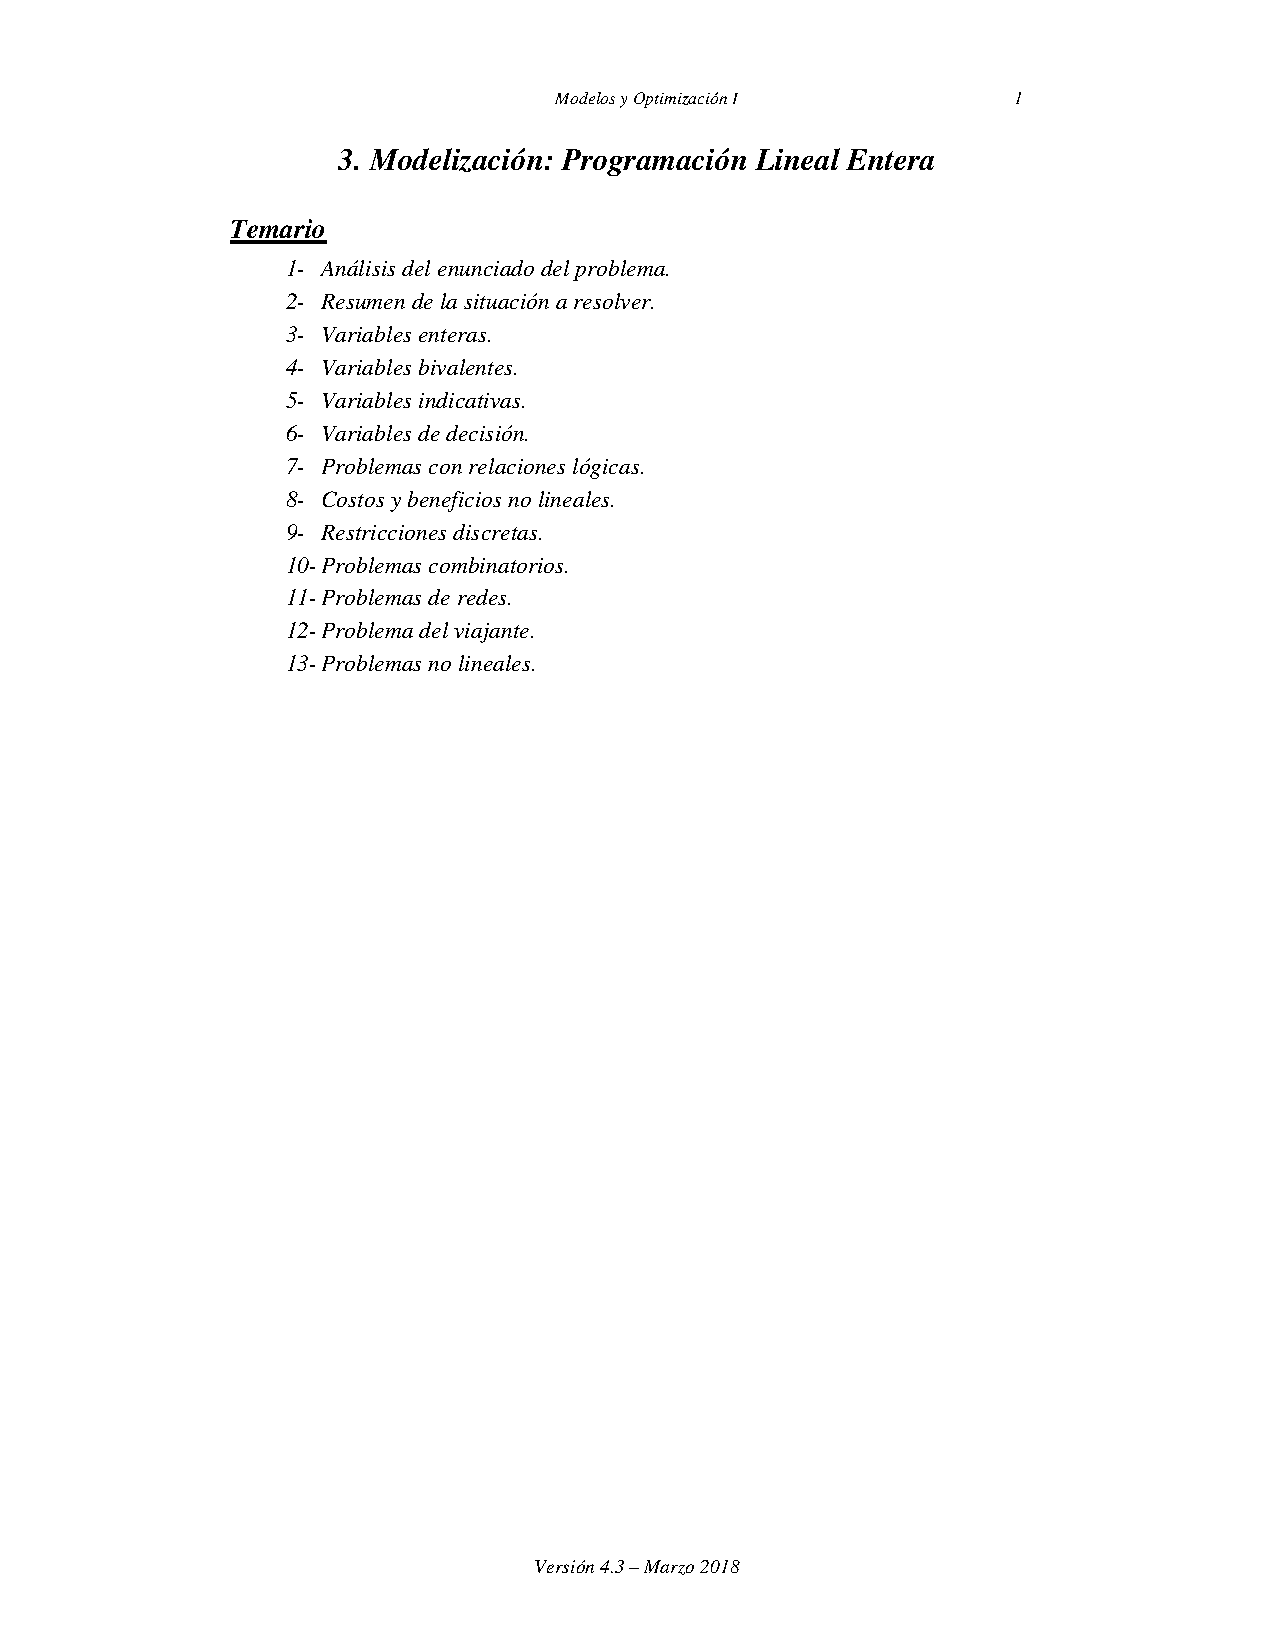
\includepdf[pages=-]{./pdfs/GuiaTP_Cap3.pdf}

\section{Resoluci\'on Guia 3}
\subsection{Ejercicio 3.3}
\begin{enumerate}[a]


\item \quad $ y_2 \geq y_1$
\item \quad $ 12 y_1 \leq MES \leq 11 + y1$ (recordar que MES es entera en rango de [1..12])
\item \quad $ Y_1 \leq Y_2 + Y_3 + Y_4 \leq 3Y_1 $ 
\item \quad $ 2Y_1 \leq Y_2 + Y_3 \leq 1 + Y_1 $ 
\item \quad $ Y_1 + Y_2 = 1 $ 
\item 
	\begin{itemize}
	\item $ E_1 =  E_1^{'} +  E_1^{''}  $
	\item $ 1 y_1 \leq E_1^{'} \leq 3 y_1 $
	\item $ 4 y_2 \leq E_1^{''} \leq 7 y_2$
	\item $ y_1 + y_2 = 1$
	\end{itemize}
\item \quad $ 10  \leq C_1 \leq M  $ 
\item \quad $ E_1 = 2 E_2 + 1$ 
\item
	\begin{itemize}
	\item $ E_1 =  E_1^{'} +  E_1^{''}  +  E_1^{'''}  $
	\item $ 4 y_1 \leq E_1^{'} \leq 4 y_1 $
	\item $ 9 y_2 \leq E_1^{''} \leq 9 y_2$
	\item $ 16 y_3 \leq E_1^{'''} \leq 16 y_3$	
	\item $ y_1 + y_2 +y_3= 1$
	\end{itemize}
\item \quad $ 50 + 25(1-y_1)\leq C_1 $
\item 
	\begin{itemize}
	\item $ E_1 =  E_1^{'} +  E_1^{''}$
	\item $ 100 y_1 \leq E_1^{'} \leq M y_1 $
	\item $ m y_2 \leq E_1^{''} \leq 80 y_2$
	\item $ y_1 + y_2 = 1$
	\end{itemize}
\end{enumerate}


\subsection{Ejercicio 3.9}
\begin{enumerate}[a]


\item 
	\begin{itemize}
	\item 	$ m Y_1 \leq C_1 \leq  M Y_1$ (con esta detecto si es mayor que cero)
	\item	$ 22 Y_1 \leq C_1 \leq M Y_1$  ( con esta me aseguro que sea mayor a 22)
	\end{itemize}

\item 
	\begin{itemize}
	\item 	$ E_2 \leq E_1 \leq  E_2 + M Y_2 $ 
	\item 	$ E_3 \leq E_1 \leq  E_3 + M Y_3 $ 
	\item 	$ E_4 \leq E_1 \leq  E_4 + M Y_4 $ 
	\item 	$ Y_2 + Y_3 + Y_4 = 2 $ 		
	\end{itemize}

\item \quad el c
\item 
	\begin{itemize}
	\item 	$ m Y_2 \leq C_2 \leq M Y_2 $ 
	\item 	$ C_1\leq M Y_2 $ 
	\end{itemize}



\item 
	\begin{itemize}
	\item $ C_1 -13 = ex - def \Rightarrow C_1$ es continua y lo comparo con el valor que no puede tomar
	\item 	$ m Y_{ex} \leq ex \leq M Y_{ex} \Rightarrow$ 	ex toma valor si C1 es mayor a 13
	\item 	$ m Y_{def} \leq def \leq M Y_{def} $ 	
	\item $ Y_{ex} + Y_{def }= 1 \Rightarrow$ con esta ecuación evito que ex = def = 0 es decir siempre tienen que ser diferentes
	\end{itemize}
\item \quad $ C_1 -1  \leq E_1 \leq C_1  $ 
\item
	\begin{itemize}
	\item $  6Y_2 \leq  E_2  \leq 5 + M Y_2 $
	\item $  6Y_3 \leq  E_3  \leq 5 + M Y_3 $
	\item $  6Y_4 \leq  E_4  \leq 5 + M Y_4 $
	\item $  6Y_5 \leq  E_5  \leq 5 + M Y_5 $
	\item $ Y_2 + Y_3 + Y_4 + Y_5 = E_1$
	\end{itemize}
\item \quad $ 50 + 25(1-y_1)\leq C_1 $
\item 
	\begin{itemize}
	\item $ E_1 =  E_1^{'} +  E_1^{''}$
	\item $ 100 y_1 \leq E_1^{'} \leq M y_1 $
	\item $ m y_2 \leq E_1^{''} \leq 80 y_2$
	\item $ y_1 + y_2 = 1$
	\end{itemize}
\end{enumerate}


\section{Resoluci\'on}
\begin{enumerate}
\item 
	\begin{enumerate}[i]
	\item \textbf{verdadero} de forma trivial.
	\item \textbf{verdadero}, Recordar que $ \{ C \subseteq D \Leftrightarrow \forall x \in C \Rightarrow x \in D \} $ y podemos ver 			que 1 esta en ambos connjuntos.
	\item \textbf{verdadero}, el razonamiento es id\'entico, solo hay que tener en cuenta que para conjuntos no es 				relevante 	ni las repeticiones de elementos ni el \'orden.
	\item \textbf{falso}, porque el conjunto cuyos \'unicos elementos son 1,3 no esta en A, $ \{ 1, 3\} \notin A $ aqui 			hay que tener en cuenta que se esta usando el pertenece y no la inclusi\'on de conjuntos.
	\item \textbf{falso} por la misma raz\'on que el item anterior.
	\end{enumerate}
\item 2
\item 3
\item 4
\item 	
	\begin{enumerate}[i]
	\item \textbf{Recordemos que} $B \vartriangle C $ son todos los elementos que estan en B o en C pero no en ambos.\\
		$B\vartriangle C = \{ 1, \{ 3 \}, 10, -2, \{1, 2, 3\}, 3 \} $ \\
		$ A\cap (B\vartriangle C ) = \{ 1, -2, 3\}$ \\ 
		
	\item $ A\cap B = \{ 1\} $ y $ A\cap C = \{ -2,3\}  \Rightarrow  (A\cap B) \vartriangle (A\cap C ) =  \{1, 					-2,3\} $ \\
	Notar que el resultado es igual que I porque $ A\cap (B\vartriangle C ) =  (A\cap B) \vartriangle (A\cap C )$
	ambos resultados son equivalentes solo hay que distribuir.\\
	
	\item \textbf{Usando la ley de De Morgan} 
	\begin{align*}
	A^{c} \cap B^c \cap C^c = (A\cup B\cup C)^c & \Rightarrow A \cup B\cup C = \{1, \{3\}, -2, 7, 10, \{1, 2, 3\}, 3\} \\
	&\Rightarrow (A\cup B\cup C) =  V  \\
	&\Rightarrow (A\cup B\cup C)^c = \lbrace \emptyset \rbrace
	\end{align*}
	
	\end{enumerate}
	\item 6
	\item 7
	\item 
	\begin{enumerate}[i]
	\item Podemos ver a la parte subrayada del gr\'afico como la uni\'on de tres conjuntos, \\
	$ A \cup \{ (A\cap C) - B\} \cup \{(B\cup C) - A \}$
	\item Este es claramente la diferencia sim\'etrica entre A y C, quitandole ademas todos lo elementos de B \\
	$ (A \bigtriangleup C) - B $
	\item Tambien lo podemos mirar como la uni\'on de tres subconjuntos \\
	$ \{ (A \cap B)-C\} \cup \{ (B \cap C)-A\} \cup \{ (A \cap C)-B\}   $
	\end{enumerate}
	
	\item 9
	\item 
		\begin{align*}
			P(A) \subseteq P(B)	\qquad &\Rightarrow \qquad A \subseteq B \\
			A \underbrace{\subseteq}_{definicion} \textit{P}(A) \qquad  &\Rightarrow \qquad A	
				\underbrace{\subseteq}_{Hip\'otesis} \textit{P}(B) \\
			\text{ Pero } P(B) \subseteq B \text{ ya que } \qquad \forall x \in P(B) \qquad &\Rightarrow \qquad x \in B \\
			&\Rightarrow A \subseteq B \\ \\
			A \subseteq B \qquad &\Rightarrow \qquad P(A) \subseteq P(B)	\\
			\forall x \in A \qquad &\Rightarrow \qquad x \in P(A) \\
			\forall x \in A \qquad &\Rightarrow \qquad x \in B \subseteq P(B) \\
			\forall x \in P(A) \qquad &\Rightarrow \qquad x \in P(B) \\
			& 	\Rightarrow P(A) \subseteq P(B)
		\end{align*}
	\item 11	
	\item 

\begin{enumerate}[i]
	\item 
\begin{enumerate}[a)]
	\item \textbf{falso}, tomar el contraejemplo, n = 2.
	\item \textbf{verdadero}, porque me dice que existe alg\'un n natural que cumple la condici\'on, no es una proposici\'on categ\'orica, sino singular.
	\item \textbf{verdadera}, porque los intervalos incluyen a todos los Naturales, $[5, + \infty] \cup [1,8]$
	\item \textbf{verdadera}, porque no es un intervalo vac\'io $ [5,8] \neq \emptyset$
	\item \textbf{verdadera}, porque cualquiera sea n, eligiendo m = n+1 se verifica la proposici\'on.
	\item \textbf{falso}, lo que me quiere decir, es que existe un n que verifica, que es menor estr\'icto para todo m, y eso es falso porque si n = 1, y m = 1 $ \Rightarrow $ 1 no es menor estricto que 1.
\end{enumerate}	
	
	\item 
	\item 
	\end{enumerate}
	\item 13				
	\item 14
	\item 15
	\item 16
	\item 17 R = {(1, 1), (1, 3), (1, 7), (3, 1), (3, 5)}
	\item %ejercicio 18

\begin{enumerate}[i)]
	\item \textbf{verdadero}
	\item \textbf{falso}, porque en el elemento (3, 2),  $2 \notin B $
	\item \textbf{verdadera}
	\item \textbf{verdadera}
	\item \textbf{verdadera}
	\item \textbf{verdadera}
\end{enumerate}	

	\item %ejercicio 19

\begin{enumerate}[i)]
	\item 	$	R = \{ (1, 1), (1, 3), (1, 5), (1, 7),(2,2),(2, 3), (2, 5), (2, 7),(3,3),(3, 5), (3, 7) \} $
	\item $	R = \{ (2, 1), (3,1) \} $
	\item $	R = \{ (2, 1), (2,3), (2,5), (2,7) \} $
	\item $	R = \{ (1, 7), (2, 5),(2,7), (3, 5), (3, 7) \} $
\end{enumerate}	

	\item %ejercicio 20
	\item %ejercicio 21
	
	\item %ejercicio 30
\textbf{Ejercicio 18}
\begin{enumerate}[i)]
	\item \textbf{No es funci\'on} porque el 1 tiene varias imagenes.
	\item \textbf{no es funci\'on} idem.
	\item \textbf{no es funci\'on}
	\item \textbf{no es funci\'on}
	\item \textbf{si es funci\'on} $ \forall x \in A \Rightarrow \ \exists ! 	\ y \in B \ \ \vert (x,y) \in R$
	\item \textbf{si es funci\'on}
\end{enumerate}	
		
\end{enumerate}
	
\chapter{Práctica 2 - Números Naturales e Inducción} 
%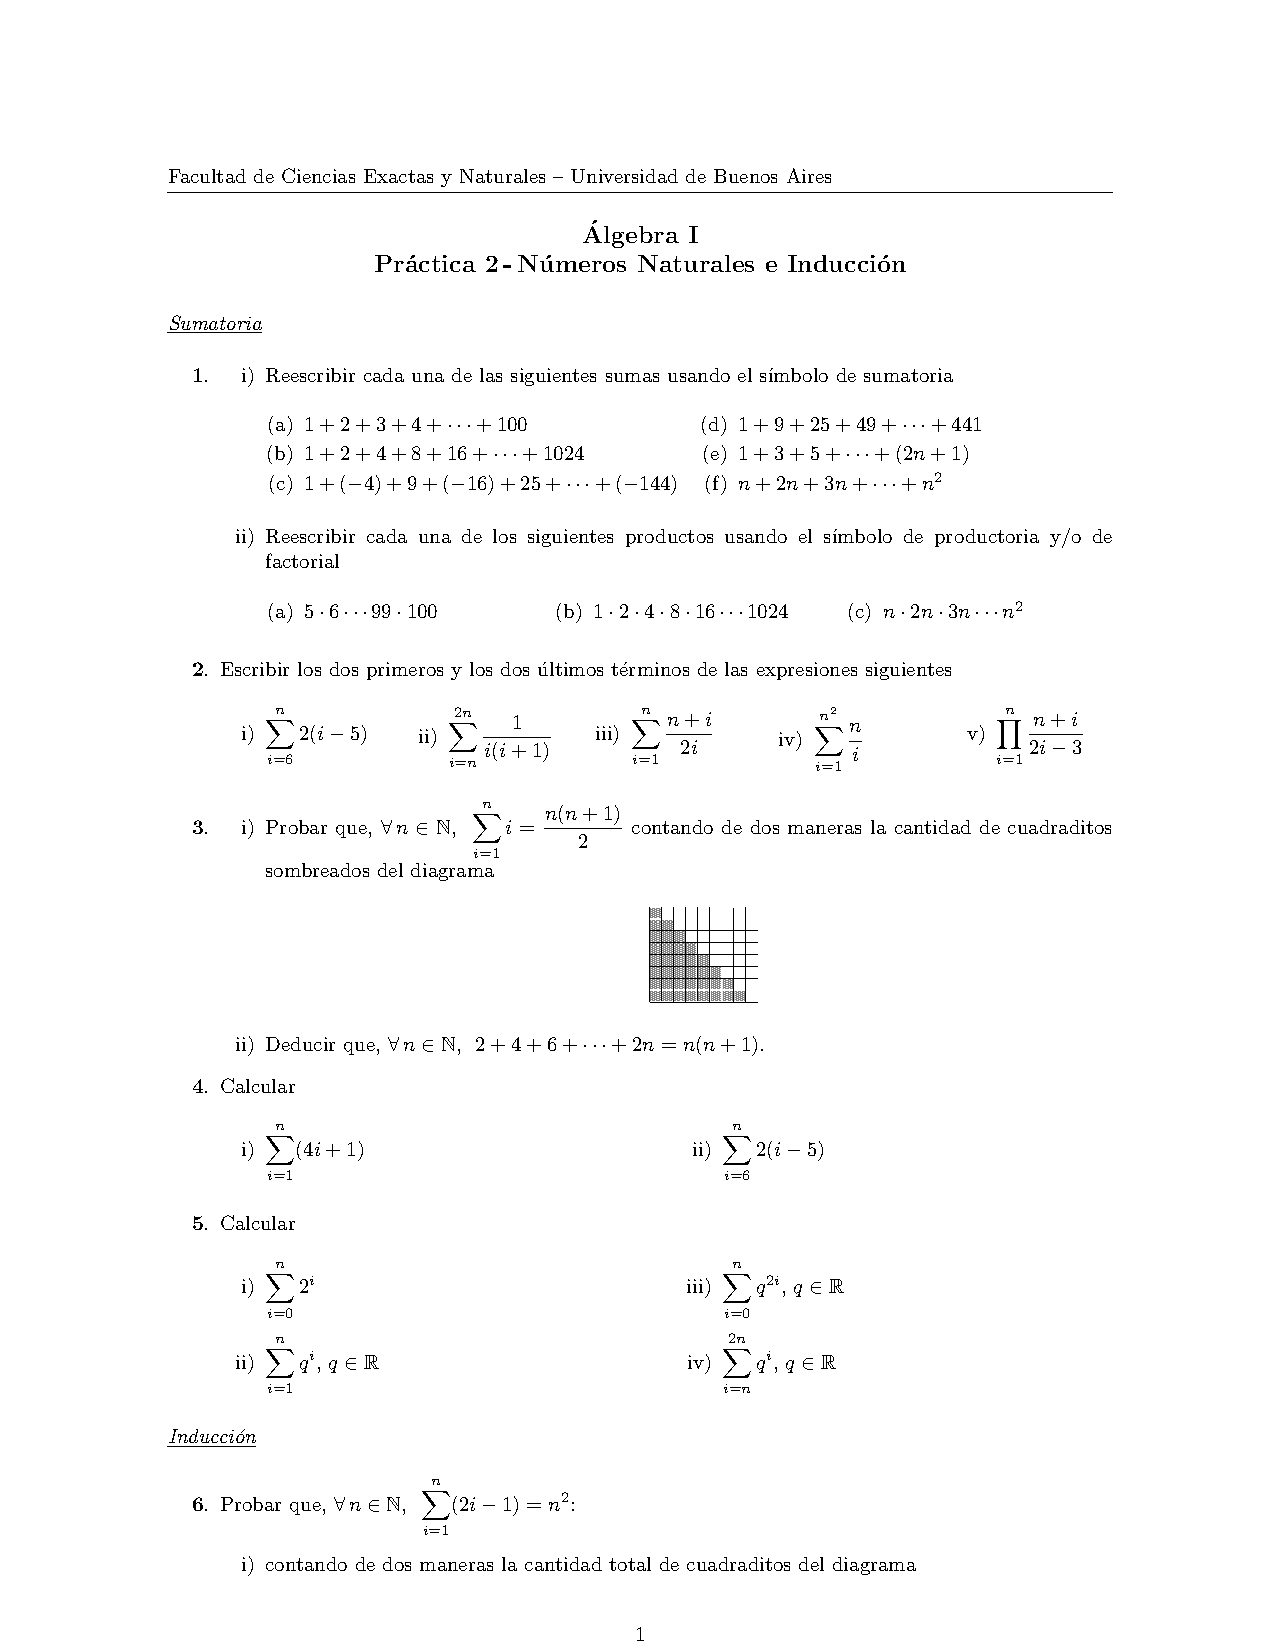
\includepdf[pages=-]{./pdfs/Practica2.pdf}


\section{Resoluci\'on}
\begin{enumerate}
\item 
	\begin{enumerate}[i)]
	\item % ejercicio 1	
	\begin{enumerate}[a)]
	\item $ \sum_{i=1}^{100}i $ \qquad (es la sumatoria trivial).
	\item $ \sum_{i=1}^{11}2^{i-1} $ 	
	\item $ \sum_{i=1}^{12}(-1)^{i-1} \cdot i^2 $		
	\item $ \sum_{i=1}^{21}(2i-1)^{2} $ 	
	\item $ \sum_{i=0}^{n}(2i+1) $ 		
	\item $ \sum_{i=1}^{n}(i\cdot n) $ 			
	\end{enumerate}
	
	
	
	\item % ejercicio 2
	
	\begin{enumerate}[a)]
	\item $ \prod_{i=5}^{100}i=5\cdot 6\cdots 100  $ 
	\item $ \prod_{i=0}^{10}2^i $ 
	\item $ \prod_{i=1}^{n}(i \cdot n) $ 	
	\end{enumerate}
	
	
	\end{enumerate}
\item %ejercicio 2
	\begin{enumerate}[i)]
	\item
\[
\sum_{i=6}^{n}2(i-5) = 2(6-5)+2(7-5)+ \cdots + 2(n-1-5)+2(n-5)
\]

	\item 

\[
\sum_{i=n}^{2n} \frac{1}{i(i+1)}= \frac{1}{n(n+1)} + \frac{1}{(n+1)(n+1+1)} + \cdots + \frac{1}{(2n-1)(2n-1+1)} + \frac{1}{2n(2n+1)}
\]
	
	\item 
\[
\sum_{i=1}^{n}\frac{n+i}{2i} = \frac{n+1}{2 \cdot 1}+\frac{n+2}{2 \cdot 2}+ \cdots + \frac{(n-1)+1}{2 \cdot (n-1)}+\frac{n+n}{2 \cdot n}
\]
	
	\item 
\[
\sum_{i=1}^{n^2}\frac{n}{i} = \frac{n}{1}+\frac{n}{2}+ \cdots + \frac{n}{(n-1)^2}+\frac{n}{n^2}
\]


	\item 
\[
\prod_{i=1}^{n}\frac{n+i}{2i-3} = \frac{n+1}{2\cdot 1-3} \cdot \frac{n+2}{2\cdot2 - 3} \cdots  \frac{n+(n-1)}{2(n-1)-3}\cdot \frac{n+n}{2n-3}
\]
		
	\end{enumerate}

\item %ejercicio 3

	\begin{enumerate}[i)]
	\item Usamos inducci\'on, primero para n=1
	\[ \sum_{i=1}^{1} i = 1 \text{ (ahora verificamos la f\'ormula ) } \frac{n(n+1)}{2} \text{, con n = 1, } \] 
	\[ \frac{1(1+1)}{2} = 1 \text{, se verifica la propiedad para n = 1. }	\Rightarrow P(1) = True\]
\\
\textbf{Hip\'otesis inductiva} \[ \sum_{i=1}^{n} i = \frac{n(n+1)}{2}\]
\\
\textbf{T\'esis inductiva} 
\begin{align*}
\sum_{i=1}^{n+1}i &= \frac{(n+1)(n+1+1)}{2} \\
\sum_{i=1}^{n+1}i &= \sum_{i=1}^{n}i + (n+1)\\
\underbrace{\sum_{i=1}^{n}i}_{\frac{n(n+1)}{2}} + (n+1) & \underbrace{=}_{ \text{por HI }} \frac{n(n+1)}{2} + (n+1) \\ \\
\frac{n(n+1)}{2} + (n+1) &= \frac{n(n+1) + 2(n+1)}{2} \qquad \text{ (factor com\'un (n+1))} \\
\frac{n(n+1) + 2(n+1)}{2} &= \frac{(n+1)(n+2)}{2} 
\end{align*}
\begin{shaded}
\[ \textbf{probamos que }\Rightarrow \sum_{i=1}^{n+1}i = \frac{(n+1)(n+1+1)}{2} \qquad \forall n \in \mathbb{N} \]
\end{shaded}
	\item De igual manera probaremos, por inducci\'on la igualdad \[ 2+4+6+\cdots+2n = \sum_{i=1}^{n} 2i = n(n+1)\] para ello probamos que cumple para n=1, $ P(1) \Rightarrow \sum_{i=1}^{1} 2i = 1(1+1) = 2$, luego probamos el paso inductivo, suponiendo que P(n) es verdadero, $\sum_{i=1}^{n} 2i = n(n+1)$ probamos que es verdadero P(n+1) o $ \sum_{i=1}^{n+1} 2i = (n+1)(n+2) $.\\
Partimos de $\sum_{i=1}^{n+1} 2i$ y trataremos de llegar l\'ogicamente a $ (n+1)(n+2) $,\\
 $ \Rightarrow \sum_{i=1}^{n+1} 2i = \sum_{i=1}^{n} 2i + 2(n+1) \text{ pero usando la HI, } n(n+1)+2(n+1)$ y sacando factor com\'un (n+1) llegamos a, $ (n+1)(n+2)$ 	que era justo lo que queriamos probar.
	\end{enumerate}

\item %ejercicio 4
\item %ejercicio 5
Se trata de una serie geom\'etrica.
\[ \sum_{i=0}^{n} 2^i = 1+2+4+6+\cdots+2^n\] si multiplico ambos miembros por 2 y resto convenientemente
\begin{align*}
 \sum_{i=0}^{n} 2^i &= 1+2+4+6+\cdots+2^n  \\
  2 \cdot (\sum_{i=0}^{n} 2^i) &= 2\cdot(1+2+4+6+\cdots+2^n) \\
  \rule{20mm}{0.2mm} &  \rule{60mm}{0.2mm} \\
 2 \cdot (\sum_{i=0}^{n} 2^i)-  (\sum_{i=0}^{n} 2^i)  &= (2+4+6+ \cdots +2^n+2^{n+1}) - (1+2+4+6+ \cdots +2^n) \\
 \sum_{i=0}^{n} 2^i &= 2^{n+1} -1
\end{align*}
\end{enumerate}


\chapter{Práctica 3 - Números enteros (Parte 2)}
\section{Guia 3}
%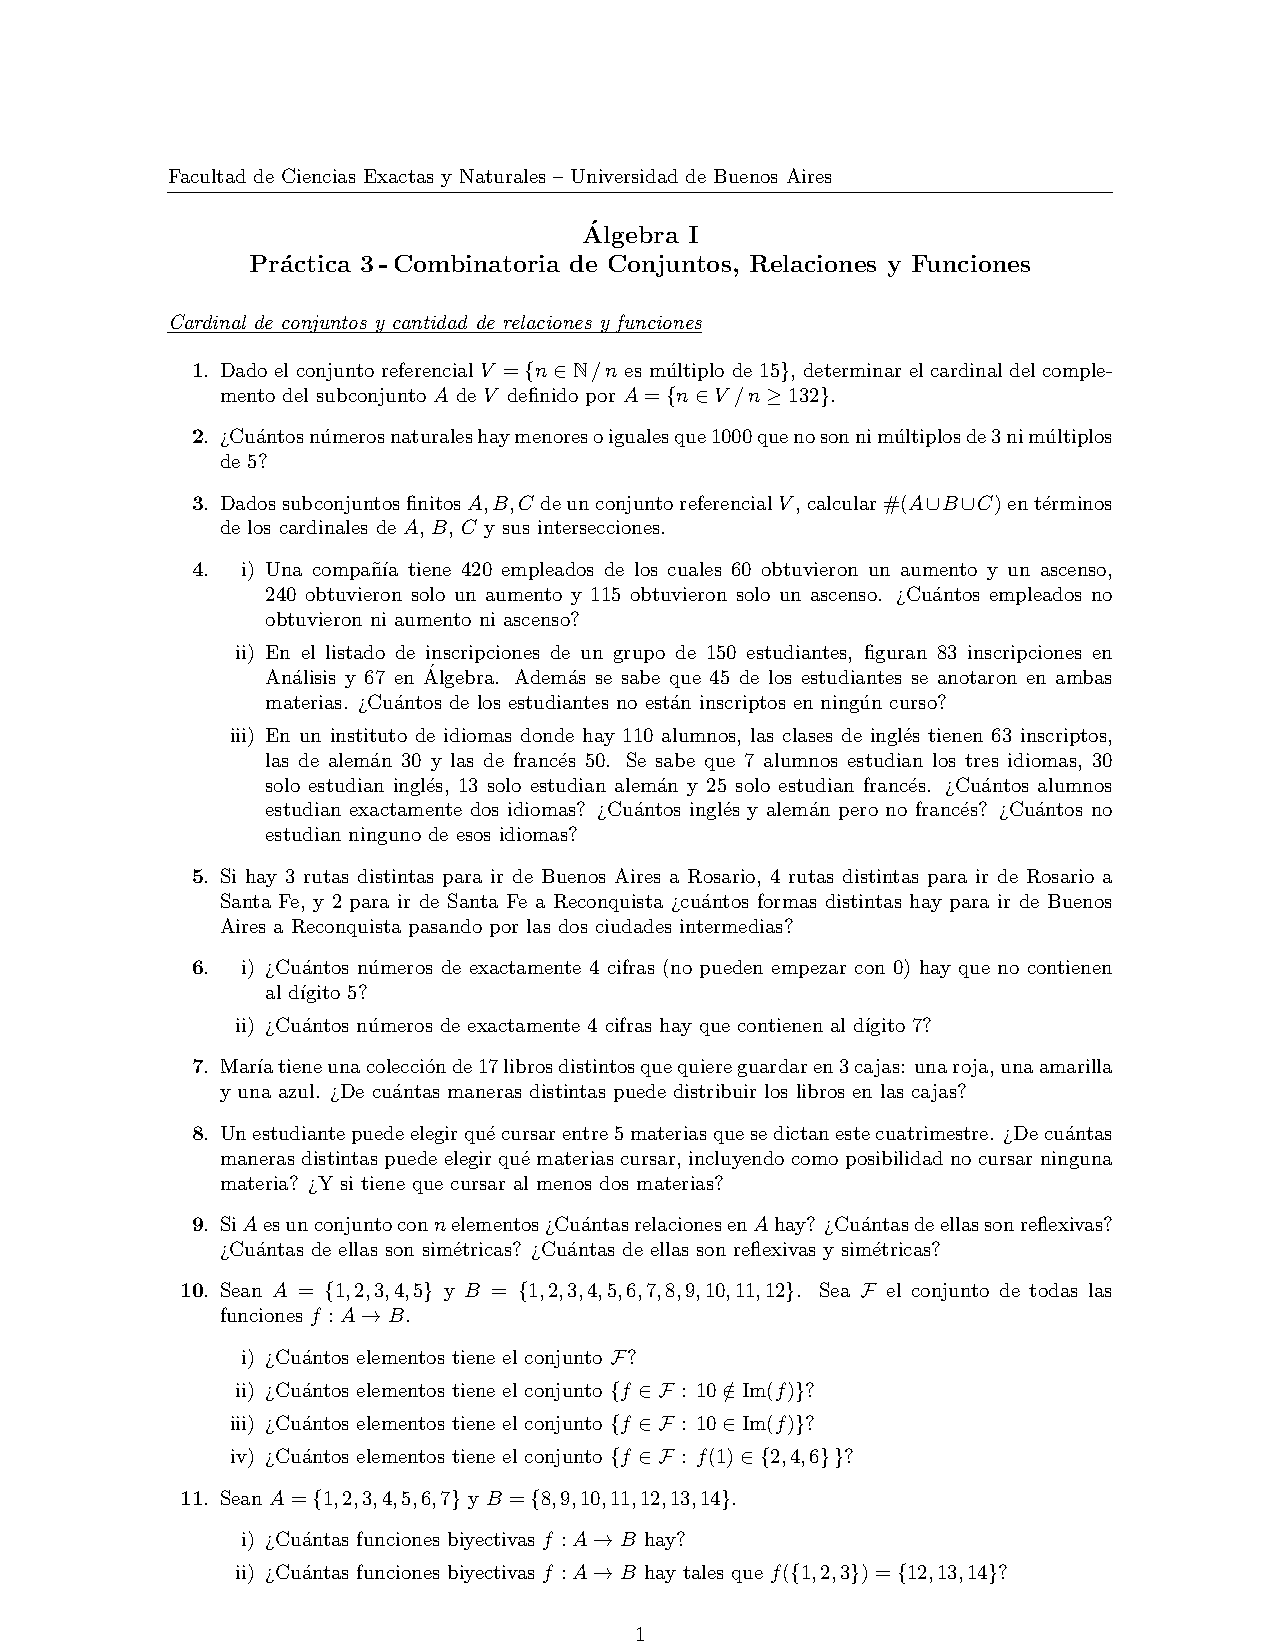
\includepdf[pages=-]{./pdfs/Practica3.pdf}


\section{Resoluci\'on}



\chapter{Práctica 4 - Números enteros (Parte 2)}
\section{Guia 4}
%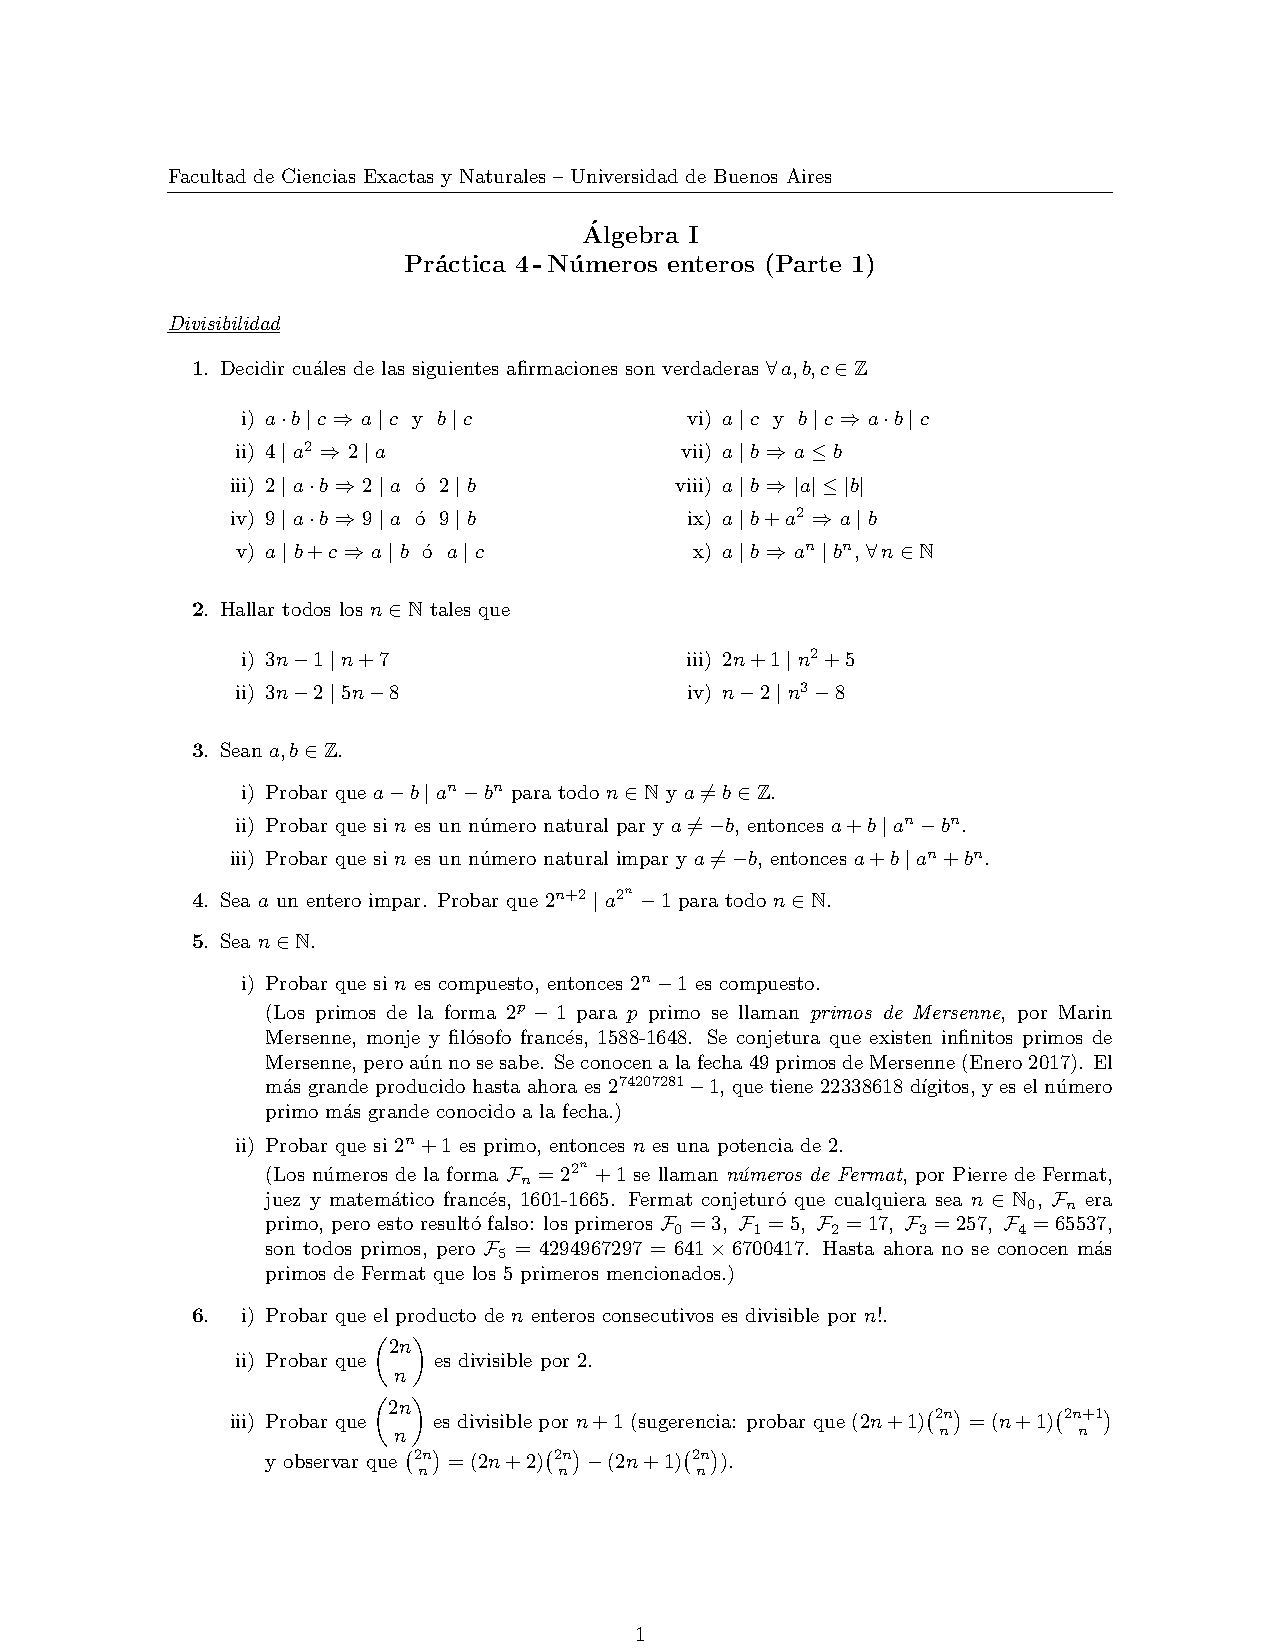
\includepdf[pages=-]{./pdfs/Practica4.pdf}


\section{Resoluci\'on}


\chapter{Práctica 5 - Números enteros (Parte 2)}
\section{Guia 5}
%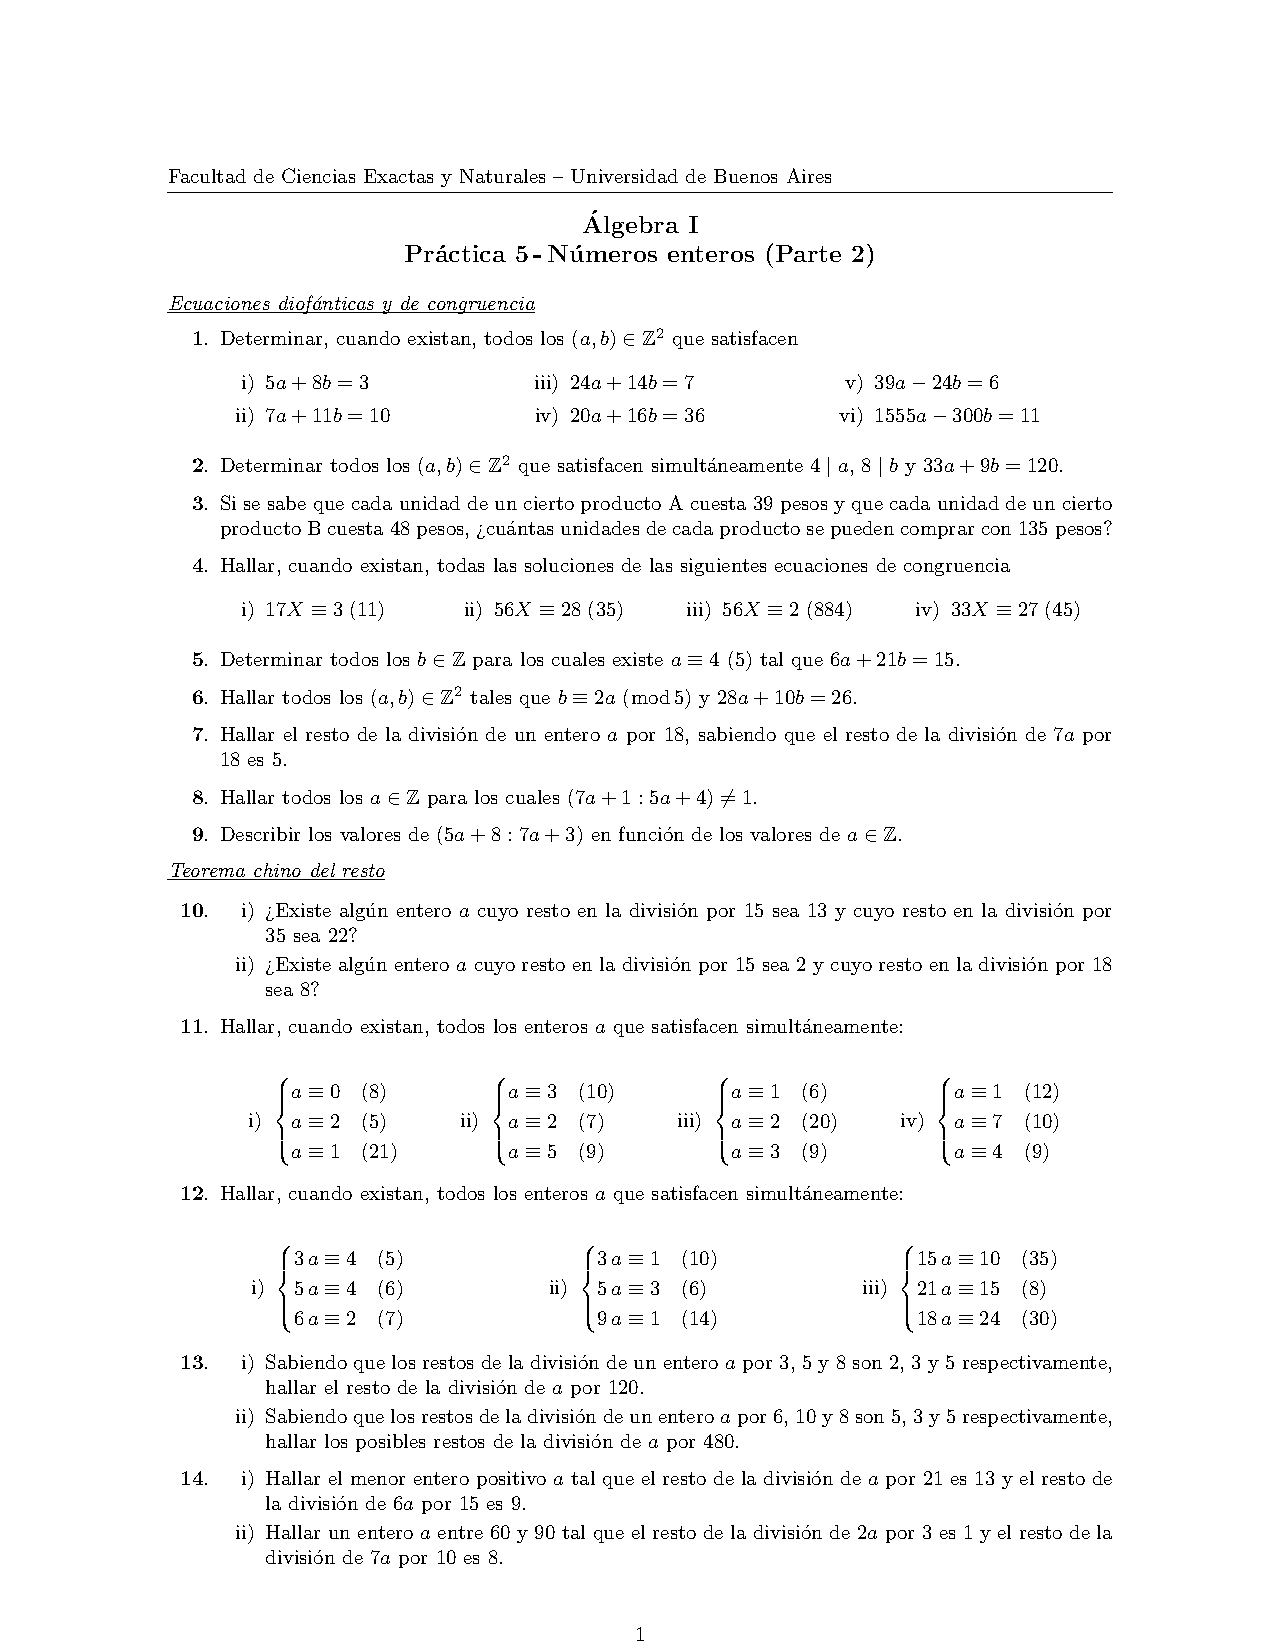
\includepdf[pages=-]{./pdfs/Practica5.pdf}


\section{Resoluci\'on}


hola mundo














\begin{shaded}
Para demostrar la corrección del programa en SmallLang con respecto a la especificación, debemos probar que:
\begin{align}
Post &\Rightarrow wp( \textbf{ c\'odigo previo al ciclo } , Pc) \\
Pc &\Rightarrow wp (\textbf{ ciclo}, Qc ) \\
Qc & \Rightarrow wp ( \textbf{ c\'odigo posterior al ciclo }, Post) 
\end{align}
La parte 2.2 con el teor\'ema del invariante. Si probamos estas tres implicaciones, por el principio de monoton\'ia sabemos que  $ Pre \Rightarrow wp(  programa completo  , Post)  $  y por lo tanto el programa  es correcto, respecto a su especificaci\'on
\end{shaded}

\section{Definici\'on de $ Qc, Pc, I, fv$}
Primero vamos a definir los predicados que necesitamos para la demostracion.
\begin{align*}
Pre & \quad \quad \{ True \}  \\
Post &= \quad \{ r = True \leftrightarrow ((\exists k :\mathbb{Z})(0 \leq k < |s|) \wedge_L s[k] = e)\} \\
Pc &= \quad (i = 0) \wedge (j = -1) \\
Qc &=  \quad(j \neq -1) \leftrightarrow (\exists k : \mathbb{Z})(0 \leq k < \mid s\mid \ \wedge_{L} \ s[k] = e) \\
I &= \quad 0 \leq i \leq  \mid s \mid) \wedge (j \neq -1) \leftrightarrow (\exists k : \mathbb{Z})(0 \leq k < i \rightarrow_L s[k] = e) \wedge (s[i] = e \rightarrow i = j)  \\
fv &= \quad ( \mid s \mid - i )\\
B &= \quad (i < \mid s \mid)
\end{align*}

\subsection{ Pre $\Rightarrow $ wp(código previo al ciclo, Pc )}
\begin{align*}
Pre \rightarrow wp(i:= 0; j := -1, Pc ) & \equiv \quad wp(i := 0; wp(j := -1, Pc )) \\ \\
Calculamos \ wp(j := -1, Pc ) & \\ 
wp(j := -1, Pc ) &\equiv \quad  def (-1) \wedge_L Pc_{-1}^j \\
 &\equiv \quad wp(j := -1, \left( (i = 0) \wedge (j = -1)\right)_{(-1)}^j ) \\
&\equiv \quad def (-1) \wedge (i = 0) \wedge (-1 = -1) \\
E1 &\equiv \quad  (i = 0) \\ \\
Calculamos \ wp(i := 0, E1) & \\
wp(i := 0, E1 ) &\equiv \quad  def (0) \wedge_L E1_{0}^i  \\
&\equiv \quad  True \wedge_L (i = 0)_{0}^i \\
&\equiv \quad (0 = 0) \\
E2 &\equiv \quad True 
\end{align*}
\begin{shaded}
Por lo tanto demostramos que: 
\begin{center}
$ Pre \Rightarrow wp( \textbf{ c\'odigo previo al ciclo } , Pc) $
\end{center}
\end{shaded}
\subsection{ Qc $\Rightarrow$ wp(if..then..else..fi, Post)}
\textbf{Recordamos la post } 
\[ Post = \{ r = True \leftrightarrow ((\exists k :\mathbb{Z})(0 \leq k < |s|) \wedge_L s[k] = e)\}  \]

Calculamos:
\begin{align*}
 wp(if ..... endif , Post) &\equiv wp(if ( j \neq -1) then \ r := True \ else \ r := False \ endif , Post)  \\
&\equiv def(j\neq -1) \wedge_L  \left[ (j \neq -1) \wedge wp(r := True , Post) \right] \vee \left[ (j = -1) \wedge wp(r := False, Post)\right]  \\
&\equiv \underbrace{def(j\neq -1)}_{\text{True}} \wedge_L \quad [ \qquad \qquad \qquad " \qquad \qquad \qquad ] \vee [\qquad \qquad \qquad " \qquad \qquad \qquad \qquad ]  \\
&\equiv (j \leq -1 \wedge wp(r := True, Post)) \vee (j = -1 \wedge wp(r := False, Post)) \\
&\equiv (j \leq -1 \wedge \textcolor{red}{wp(r := True, Post)}) \vee (j = -1 \wedge \textcolor{blue}{ wp(r := False, Post)}) 
\end{align*}
\begin{align*}
\textcolor{red}{wp(r := True, Post)} &\equiv def (True) \wedge_L Post_{true}^r \\
&\equiv (True = True) \leftrightarrow (\exists k : \mathbb{Z})(0 \leq k < |s| \wedge_L s[k] = e) \\
\textcolor{red}{wp(r := True, Post)} &\equiv (\exists k : \mathbb{Z})(0 \leq k < |s| \wedge_L s[k] = e) \\ \\  \\
\textcolor{blue}{ wp(r := False, Post)} &\equiv def (False) \wedge_L Post_{false}^r \\
&\equiv \underbrace{(false = True)}_{\text{False}} \leftrightarrow \underbrace{(\exists k : \mathbb{Z})(0 \leq k < |s| \wedge_L s[k] = e)}_{\text{(*)}} \\
(*) \ entonces \ como \ & (\exists k : \mathbb{Z})(0 \leq k < |s| \wedge_L s[k] = e)  \text{ debe ser Falso,  invierto desigualdad} \\ \\
\textcolor{blue}{ wp(r := False, Post)} &\equiv (\forall k : \mathbb{Z})(0 \leq k < |s| \wedge_L s[k] \neq e)\\ \\ \\ \\
wp(if... endif , Post) &\equiv (j \neq -1) \wedge ( \exists k : \mathbb{Z})(0 \leq k < |s| \wedge_L
s[k] = e) \vee \\ 
& \quad \ (j = -1) \wedge (\forall k :\mathbb{Z})(0 \leq k < |s| \wedge_L s[k] \neq e) \\
& \quad \ \textcolor{blue}{(aplico \ (p \wedge q) \vee (\neg p \wedge \neg q) \equiv p \leftrightarrow q)} \\
E3 &\equiv (j \neq -1) \leftrightarrow (\exists k :\mathbb{Z})(0 \leq k < |s| \wedge_L s[k] = e) 
\end{align*}
Chequeamos $Qc \rightarrow E3 $ 
\begin{align*}
Qc \equiv j \neq -1 & \leftrightarrow (\exists k : \mathbb{Z})(0 \leq k < |s| \wedge_L s[k] = e) \equiv E3
\end{align*}
\begin{shaded}
Por lo tanto demostramos que: 
\begin{center}
$Qc \Rightarrow E3$ 
\end{center}
\end{shaded}
\chapter{Demostraci\'on de la correcci\'on del ciclo}
\subsection{Qc $\Rightarrow$ wp(ciclo, Qc)}
\begin{shaded}
\textbf{Teorema}. Sean un predicado I y una funci\'on $ fv : \mathbb{V} \rightarrow \mathbb{Z} $
(donde $ \mathbb{V} $ es el producto cartesiano de los dominios de las variables del programa), y supongamos que I $ \rightarrow $ def(B). Si se cumplen: \\
\begin{align*}
\textbf{1)}\quad & PC \Rightarrow I, \\
\textbf{2)}\quad & \{I \wedge B \} S \{I \}, \\
\textbf{3)}\quad & I \wedge \neg B \Rightarrow Qc , \\
\textbf{4)}\quad & \{I \wedge B \wedge v_0 = fv \} S \{fv < v_0 \}, \\
\textbf{5)}\quad & I \wedge fv \leq 0 \Rightarrow \neg B, 
\end{align*}
... entonces la siguiente tripla de Hoare es v\'alida: \{PC \} while B do S endwhile \{QC \}
\end{shaded}
\subsection{$ Pc \ \rightarrow I $}
\begin{align*}
Pc &= \quad (i = 0) \wedge (j = -1) \\
I &= \quad 0 \leq i \leq  \mid s \mid) \wedge (j \neq -1) \leftrightarrow (\exists k : \mathbb{Z})(0 \leq k < i \rightarrow_L s[k] = e) \wedge (s[i] = e \rightarrow i = j) \\
&\equiv \quad (i = 0) \wedge (j = -1) \rightarrow ( 0 \leq i \leq  \mid s \mid) \  \checkmark (\textcolor{red}{trivial }) \\
&\equiv \quad (j\neq -1 \land (\exists k: \mathbb{Z})  ( 0\leq k <i \land_L s[k] = e ))  \lor  (j= -1 \land (\forall k: \mathbb{Z})  ( 0\leq k < i \land_L s[k] \neq e )) \checkmark 	
\end{align*}
( \textcolor{red}{porque  se cumple trivialmente que $ (j = -1) $ y por vacuidad $(j= -1 \land (\forall k: \mathbb{Z})  ( 0\leq k < i \land_L s[k] \neq e ))$ ya que no hay ningún número que sea mayor o igual a cero y menor a cero a la vez  }) 
\vspace{0.3cm}
\subsection{ $ (I \ \land \neg B) \rightarrow Qc$ }

\begin{align*}
Q_c &\equiv (j \neq -1)  \Leftrightarrow (\exists k: \mathbb{Z})(0 \leq k < |s| \land_L s[k] = e)  \\
B   &\equiv (i < |s|) \\
I &\equiv 0 \leq i \leq |s| \land j\neq -1 \Leftrightarrow (\exists k:\mathbb{Z})(0\leq k < i \Rightarrow_L s[k] = e)\wedge (s[i] = e \rightarrow i = j) \\ \\
& Q_c \checkmark 
\end{align*}
( \textcolor{red}{porque $I\land \neg B$ implica que $i = |s|$ ya que por $I $,  $ i \leq |s|$ y por $\neg B$\, $i \geq |s| $ y si aplico esto a $I$ me queda $Q_c$ }) 
\vspace{0.2cm}
\subsection{ \{$I\land B$\} ciclo  \{$I$\} }
\begin{align*}
I &= \quad (0 \leq i \leq  \mid s \mid) \wedge (j \neq -1) \leftrightarrow (\exists k : \mathbb{Z})(0 \leq k < i \rightarrow_L s[k] = e) \wedge (s[i] = e \rightarrow i = j) \\
B &\equiv \quad  (i < |s|) \\
\end{align*}
\begin{shaded}
\begin{align*}
& \textbf{Ciclo} \\
& \qquad if (s[i] = e)  then  \\
& \qquad \qquad j:= i \\
& \qquad else \\
& \qquad \qquad skip \\
& \qquad endif \\
& \qquad i:= i + 1 
\end{align*}
\end{shaded}
Veamos si $ (I \land B) \Rightarrow wp( $if...then..else..fi,  $ i := i +1, I ) $

\begin{align*}
wp( if..fi,   i := i +1, I )  \ &\equiv \ wp( if..fi,  \underbrace{ wp( i := i +1, I)}_{debo \ calcular} ) \\ \\
wp( i := i +1, I) \ &\equiv \  \underbrace{def(i+1)}_{True} \land_L I_{i+1}^i \\
&\equiv  (0\leq i +1 \leq|s|) \land_L ( j\neq -1 \Leftrightarrow (\exists k: \mathbb{Z})) ( 0 \leq k < i + 1 \Rightarrow_L s[k] = e)) \wedge \\
& \quad \ (s[i+1] = e \rightarrow i+1 = j)  \\ \\
E4 &\equiv  (0\leq i +1 \leq|s|) \land_L ( j\neq -1 \Leftrightarrow (\exists k: \mathbb{Z})) ( 0 \leq k < i + 1 \Rightarrow_L s[k] = e))\wedge \\
& \quad \  (s[i+1] = e \rightarrow i+1 = j)  \\
\end{align*}
\textbf{Calculo} $wp( if...then..else..fi,  E4 )$ \\
\begin{align*}
wp( if..fi,  E4 ) &\equiv \underbrace{ def(s[i] = e )}_{True} \land_L 
 \ \left[ \ s[i] = e \land wp(j := i, E4)  \ \right] \lor \left[ \ s[i] \neq e \land wp(skip, E_4)\right] \\
&\equiv (s[i] = e \land \underbrace{ def(i)}_{True} \land {E4}^j_i) \lor (s[i] \neq e \land E4) \\
&\equiv (s[i] = e \land  {E4}^j_i) \lor (s[i] \neq e \land E4) \\
&\equiv  (s[i] = e ) \quad \land  \\ 
& \quad \ (0\leq i +1 \leq|s|) \land_L ( i \neq -1 \Leftrightarrow (\exists k: \mathbb{Z})) ( 0 \leq k < i + 1 \Rightarrow_L s[k] = e))\wedge \\
& \quad \  (s[i+1] = e \rightarrow i+1 = i) \qquad \lor \\ 
& \quad \ (s[i] \neq e) \quad  \land \\
& \quad \ (0\leq i +1 \leq|s| \land_L ( j\neq -1 \Leftrightarrow (\exists k: \mathbb{Z}) ( 0 \leq k \leq i + 1 \Rightarrow_L s[k] = e))\wedge \\
& \quad \  (s[i+1] = e \rightarrow i+1 = j) \\ \\ \\
E5 &\equiv ( 0\leq i +1 \leq|s|) \land_L  \\
& \quad \ (s[i] = e \land (i\neq -1 \Leftrightarrow (\exists k: \mathbb{Z}) ( 0 \leq k < i + 1 \Rightarrow_L s[k] = e)) \wedge \\
& \quad \  (s[i+1] = e \rightarrow i+1 = i))\\
& \quad \ \lor \\  
& \quad \ (s[i] \neq e \land ( j\neq -1 \Leftrightarrow (\exists k: \mathbb{Z}) ( 0 \leq k \leq i + 1 \Rightarrow_L s[k] = e)) \wedge \\
& \quad \  (s[i+1] = e \rightarrow i+1 = j) ) \\ \\
\text{ Segun el invariante } & (s[i] = e \rightarrow i = j), \text{y usando la equivalencia }(p \wedge q )\vee(\neg p \wedge q )\equiv q \\ \\
E5 &\equiv ( 0\leq i +1 \leq|s|) \land_L  \\
& \quad \ ( \underbrace{ s[i] = e }_{\text{por I}}\land (\underbrace{ i \neq -1}_{\text{i=j}} \Leftrightarrow (\exists k: \mathbb{Z}) ( 0 \leq k < i + 1 \Rightarrow_L s[k] = e)) \wedge \\
& \quad \  (s[i+1] = e \rightarrow \underbrace{ i+1 = i }_{i=j}) )\\
& \quad \   \lor \\  
& \quad \ (s[i] \neq e \land ( j\neq -1 \Leftrightarrow (\exists k: \mathbb{Z}) ( 0 \leq k \leq i + 1 \Rightarrow_L s[k] = e)) \wedge \\
& \quad \  (s[i+1] = e \rightarrow i+1 = j) )\\ \\
E5 &\equiv ( 0\leq i +1 \leq|s|) \land_L  \\
& \quad \ ( s[i] = e \land ( j \neq -1 \Leftrightarrow (\exists k: \mathbb{Z}) ( 0 \leq k < i + 1 \Rightarrow_L s[k] = e)) \wedge \\
& \quad \  (s[i+1] = e \rightarrow i+1 = j ) )\\
& \quad \   \lor \\  
& \quad \ (s[i] \neq e \land ( j\neq -1 \Leftrightarrow (\exists k: \mathbb{Z}) ( 0 \leq k \leq i + 1 \Rightarrow_L s[k] = e)) \wedge \\
& \quad \  (s[i+1] = e \rightarrow i+1 = j) )
\end{align*}
\begin{align*}
& \textcolor{blue}{ usando (p \wedge q )\vee(\neg p \wedge q ) \equiv q } \\
E5 &\equiv ( 0\leq i +1 \leq|s|) \land_L \\
& \quad \  (j\neq -1 \Leftrightarrow (\exists k: \mathbb{Z}) ( 0 \leq k < i + 1 \Rightarrow_L s[k] = e) \wedge \\
& \quad \  (s[i+1] = e \rightarrow i+1 = j) 
\end{align*}
Ahora veamos si $ \{I \land B \} \Rightarrow E5 $ \\ \\ \\
\textbf{Hip\'otesis:}
\begin{enumerate}
\item $ B \equiv \quad  (i < |s|) $
\item $ I = \quad (0 \leq i \leq  \mid s \mid) $
\item $ \qquad \quad (j \neq -1) \leftrightarrow (\exists k : \mathbb{Z})(0 \leq k < i \rightarrow_L s[k] = e) $
\item $ \qquad \quad  (s[i] = e \rightarrow i = j)$
\end{enumerate}
\textbf{T\'esis}
\begin{enumerate}
\item $ ( 0\leq i +1 \leq|s|) $
\item $ (j\neq -1 \Leftrightarrow (\exists k: \mathbb{Z}) ( 0 \leq k < i + 1 \Rightarrow_L s[k] = e)$
\item $ (s[i+1] = e \rightarrow i+1 = j) $
\end{enumerate}
\begin{shaded}
Comenzamos por la t\'esis 1 $ ( 0\leq i +1 \leq|s|) $
\end{shaded}
\begin{align*}
\textbf{segun la hip 2 } &\Rightarrow \qquad 0 \leq i \\ 
&\Rightarrow \qquad 0 \leq i+1 \\
\textbf{segun la hip 1 } &\Rightarrow \qquad i < |s| \\ 
&\Rightarrow \qquad i+1 < |s|+1 \\
&\Rightarrow \qquad i +1 \leq |s| \\
\end{align*}
\begin{shaded}
Por lo tanto se cumple la t\'esis 1 $ ( 0\leq i +1 \leq|s|) $
\end{shaded}
\begin{shaded}
Continuamos por la t\'esis 2 \\
\[ (j\neq -1 \Leftrightarrow (\exists k: \mathbb{Z}) ( 0 \leq k < i + 1 \Rightarrow_L s[k] = e) \]
\end{shaded}
\begin{align*}
 0 \leq k < i + 1 \qquad  &\equiv \qquad  0 \leq k \leq i \\
\textbf{sabemos que } \quad i  < |s| \qquad  &\equiv \qquad  0 \leq k \leq i < |s|\\
\textcolor{blue}{(*)} &\equiv \qquad   0 \leq k  < |s|\\
(j\neq -1 \Leftrightarrow (\exists k: \mathbb{Z}) ( 0 \leq k < i + 1 \Rightarrow_L s[k] = e) & \equiv  (j\neq -1 \Leftrightarrow (\exists k: \mathbb{Z}) ( \underbrace{ 0 \leq k < |s|}_{\textcolor{blue}{(*)}} \Rightarrow_L s[k] = e) \\
& \equiv  (j\neq -1 \Leftrightarrow (\exists k: \mathbb{Z}) (  0 \leq k < |s| \Rightarrow_L s[k] = e)
\end{align*}
Esto significa que j sera distinto de -1 cuando exista un k que estando en rango verifique que el elemento en la posicion k sea e, y sera falso cuando e no este en la secuencia.

\begin{shaded}
Continuamos por la t\'esis 3 \[ (s[i+1] = e \leftrightarrow i+1 = j) \]
\end{shaded}
\begin{align*}
\textbf{segun la hip 4 } \quad i = j \quad   &\leftrightarrow \quad s[i] = e \\ 
&\leftrightarrow \quad  s[j] = e \\
\textbf{ pero si } \quad  j =i+1 \quad   &\leftrightarrow \quad  s[i+1] = e \\
\textbf{ de igual forma si} \quad  s[i] = e  \quad   &\leftrightarrow \quad j=i \\
s[i+1] = e  \quad   &\leftrightarrow \quad j=i+1 
\end{align*}
Esto dice que si e esta en la posicion i+1, entonces j debe ser i+1, ya que j era igual a i.

\begin{shaded}
Por lo tanto se cumple  \[ (s[i+1] = e \leftrightarrow i+1 = j) \]
\end{shaded}


\subsection{$ I \land  f_v \leq 0 \rightarrow \neg B$ }

Queremos demostrar que cuando la funci\'on variante llega a un valor determinado entonces se termina el ciclo o dicho de otra forma la guarda se hace falsa.
\begin{align*}
\textbf{Hip\'otesis} \\
I &= \quad (0 \leq i \leq  \mid s \mid) \wedge (j \neq -1) \leftrightarrow (\exists k : \mathbb{Z})(0 \leq k < i \rightarrow_L s[k] = e) \wedge (s[i] = e \rightarrow i = j) \\
fv &= \quad ( \mid s \mid - i )\leq 0  \\ \\
\textbf{T\'esis} \\
\neg B &\equiv \quad  (i \geq |s|) \\ \\ \\
\textbf{Demostraci\'on } \\
fv &\equiv \quad  \mid s \mid - i \leq 0  \\
&\equiv \quad  \mid s \mid \leq i \\
&\equiv \quad  (i \geq |s|) \qquad (\textbf{ que es } \neg B)
\end{align*}

\begin{shaded}
Por lo tanto se cumple la t\'esis $ (I \land  f_v \leq 0) \rightarrow \neg B$
\end{shaded}

\subsection{$ \{ I \wedge B \wedge v_0 = fv \}  S \{fv < v_0 \}$ }
Finalemente vamos a demostrar que la funcion variante decrece, esto equivale a decir que si estamos al principio del ciclo en donde valen, tanto el invariante, la guarda y donde la funcion variante toma cierto valor $v_0$, despues de ejecutar el cuerpo del ciclo la fv va a tomar un valor estrictamente menor a $v_0 $ .
\begin{shaded}
\begin{align*}
& \textbf{Ciclo} \\
& \ \textbf{S1}if (s[i] = e)  then  \\
& \qquad \qquad j:= i \\
& \qquad else \\
& \qquad \qquad skip \\
& \qquad endif \\
& \ \textbf{S2} i:= i + 1 
\end{align*}
Si llamamos \textbf{S1 al if..endif} y \textbf{S2 a i:=i+1}. 
Debemos hallar $wp (S1;S2, fv < v_0) $
\end{shaded}
\begin{align*}
wp (S1;S2, fv < v_0)\quad & \equiv \quad wp (S1, \ \textcolor{blue}{wp (S2, |s|-i < v_0)}) \\ \\
\textcolor{blue}{wp (S2, |s|-i < v_0)} \quad & \equiv \quad wp (i:= i + 1 , |s|-i < v_0) \\
& \equiv \quad \underbrace{ def( i + 1)}_{True} \wedge_L (|s|-i < v_0)_{i+1}^i \\
& \equiv \quad (|s|-i < v_0)_{i+1}^i \\
E2 \equiv \textcolor{blue}{wp (S2, |s|-i < v_0)}\quad  & \equiv \quad (|s|-(i+1) < v_0)
\end{align*}
Calculamos la precondici\'on m\'as d\'ebil del if..fi respecto de E2.
\begin{align*}
wp (S1,E2) \quad & \equiv \quad wp (if..fi ,E2)  \\
&\equiv \underbrace{ def(s[i] = e )}_{True} \land_L 
 \ \left[ \ s[i] = e \land wp(j := i, E2)  \ \right] \lor \left[ \ s[i] \neq e \land wp(skip, E2)\right] \\
&\equiv  \left[ \ s[i] = e \land wp(j := i, E2)  \ \right] \lor \left[ \ s[i] \neq e \land  E2 \right] \\
&\equiv ( \ s[i] = e \land (def(i) \wedge_L E2_i^j)  \ ) \lor ( \ s[i] \neq e \land  E2 ) \\
&\equiv ( \ s[i] = e \land ( E2_i^j)  \ ) \lor ( \ s[i] \neq e \land  E2 ) \\
&\equiv ( \ s[i] = e \land (|s|-(i+1) < v_0)  \ ) \lor ( \ s[i] \neq e \land (|s|-(i+1) < v_0) ) \\
& \textcolor{blue}{ usando (p \wedge q )\vee(\neg p \wedge q ) \equiv q } \\
E1 &\equiv (|s|-(i+1) < v_0) \\
E1 &\equiv (|s|-i-1 < v_0) \\
\end{align*}
Por lo tanto la precondici\'on m\'as d\'ebil que queriamos calular es E1, ahora debemos verificar que 
\[ \{ I \wedge B \wedge v_0 = fv \}  \Rightarrow E1 \]
\begin{align*}
fv \quad &= \quad  v_0   \\
|s|-i \quad &= \quad  v_0   \qquad (\text{ restando 1 a ambos miembros obtenemos}) \\
|s|-i -1 \quad &= \quad  v_0  -1 \qquad (\text{ pero $ (v_0-1) < v_0$}) \\
|s|-i -1 \quad &= \quad  v_0  -1 < v_0\\
|s|-i -1 \quad &< \quad  v_0
\end{align*}

\begin{shaded}
Por lo tanto nuestra funcion variante decrece y \[ \{ I \wedge B \wedge v_0 = fv \}  \Rightarrow E1 \]
\end{shaded}

\chapter{Conclusiones}
Estamos en condiciones de afirmar que nuestro programa, habiendo demostrado a través del teorema de invarinate que el ciclo es correcto respecto de su espeficicaci\'on y a través del teorema de terminacion del ciclo, que el mismo finaliza siempre y ademas termina en un estado en que vale la postcondicion del ciclo. \\
Con todo esto probado y por el principio de monotonia probamos que el programa completo es correcto respecto de la especificaci\'on dada.
\end{document}


